\documentclass[a4paper,11pt,psamsfonts,reqno]{amsart}

\usepackage[utf8]{inputenc}
\usepackage[T1]{fontenc}
\usepackage[english]{babel}
\usepackage{calc}
\usepackage{color}
\usepackage{float}
\usepackage{geometry}
\usepackage{microtype}
\usepackage{setspace}
\usepackage{graphicx}
\usepackage[colorlinks=true,urlcolor=blue]{hyperref}
\usepackage{longtable}
\usepackage{pdfpages}
\usepackage{amscd,amsmath,amssymb,amstext,amsthm}
\usepackage{braket}
\usepackage{mathpartir}
\usepackage{tikz}

\usetikzlibrary{cd}
\usetikzlibrary{patterns}


\geometry{a4paper,left=20mm,right=20mm,top=20mm,bottom=20mm}
\onehalfspacing

\allowdisplaybreaks


\newcounter{prpcounter}


\newtheoremstyle{proposition}
{0pt}
{10pt}
{\normalfont}
{}
{\bfseries}
{}
{0.8em}
{\bfseries{\thmnumber{#2}\hspace{0.4em}\thmname{#1}\thmnote{\hspace{0.5em}(#3)}}}

\newtheoremstyle{proof}
{0pt}
{10pt}
{\normalfont}
{}
{\bfseries}
{}
{0.8em}
{\bfseries{\thmname{#1}\thmnote{\hspace{0.5em}(#3)}}}


\theoremstyle{proposition}
\newtheorem{prp}{Proposition}[prpcounter]
\newtheorem{con}[prp]{Conjecture}
\newtheorem{cor}[prp]{Corollary}
\newtheorem{cst}[prp]{Construction}
\newtheorem{exa}[prp]{Example}
\newtheorem{lem}[prp]{Lemma}
\newtheorem{rem}[prp]{Remark}
\newtheorem{thm}[prp]{Theorem}


\theoremstyle{proof}
\newtheorem{prf}{Proof}


\begin{document}

\title{a primer on topological insulators}
\author{SHTSoft.EU}
\date{\today}
\maketitle
\tableofcontents

\setcounter{prpcounter}{0}


\input{macros.tex}


\section{Introduction}
\label{sec:intro}
\stepcounter{prpcounter}
\nocite{eda79af1}
\nocite{fd8cbb36}
\nocite{1706ae98}
The 2016 Nobel laureates in physics are Thouless, Haldane and Kosterlitz {\glqq}for the theoretical discoveries of topological phase transitions and topological phases of matter{\grqq} as officially stated by the Nobel Foundation. Shortly after von Klitzing in 1980 observed a quantized Hall conductance of a two dimensional system of electrons at nearly zero temperature in a perpendicular magnetic field, the 2016 Nobel laureates made it to show that these very robust quantization does not merely have its origin in ordinary quantum mechanics but rather in the topology of the spectrum.
\\
Von Klitzing found for the Hall conductance that
\begin{align*}
  \sigma
  &=
  \frac{e^{2}}{h}
  \nu
  ,\qquad
  \nu
  \in
  \mathbb{N}
\end{align*}
where $e$ is the elementary charge and $h$ is Planck's constant. $\nu$ is an integer depending monotonously on the strength of the magnetic field and is zero for a disappearing magnetic field. Consequently, one calls the effect above the \textit{integer quantum Hall effect (IQHE)}. It turned out that $\nu$ was well-known topological invariant of the spectrum related to K-theory making the IQHE the historically (compare \cite{1706ae98}) first type of a topological phase distinction. If the IQHE is exhibited in a solid insulator the insulator is called topological insulator.
\\
The theory of topological insulators is a young field of research that utilizes many mathematical theories which is probably the reason why there are not so many convenient ways to get in touch with it - for the common undergraduate student, at least. The paper's main purpose is to make up for this serving as an accessible introduction to topological insulators.
\\
The paper is structured as follows
\begin{enumerate}
\item[$\bullet$]
Section \ref{sec:mathpre} discusses the mathematical background needed to get a rough understanding of toplogical insulators. The ultimate ambition of section \ref{sec:mathpre} is to tool up the reader with topological K-theory which, in some limited cases, allows describing topological insulators.
\item[$\bullet$]
Section \ref{sec:topins} tries to convey a high-level picture of topological insulators. We will start out saying what we mean by insulator precisely. After that, we briefly outline the general K-theoretic classification of topological phases. The section culminates in the somewhat famous periodic table for topological insulators proposed in \cite{eda79af1} by Kitaev as well as the high-level presentation of the IQHE and more general Chern insulators which are contained in this periodic table.
\item[$\bullet$]
Section \ref{sec:kmm} - the last section - concerns the Kane-Mele model on a lower-level. It is a model for another kind of (two-dimensional) topological insulators contained in Kitaev's periodic table. To put it in a nutshell we use methods similar to that of section \ref{sec:topins} to describe the model and to find a topological invariant like the integer in the IQHE. It will be explicit enough to implement it as opposed to the dicussion in section \ref{sec:topins}.
\end{enumerate}



\section{Mathematical Preliminaries}
\label{sec:mathpre}
\stepcounter{prpcounter}
\nocite{8b5861fc}
\nocite{c7f15065}
In this section we recount the mathematics needed to receive an impression of topological insulators. The mathematical branches relevant for the theory of topological insulators
\begin{enumerate}
\item[$\bullet$]
  (functional) analysis
\item[$\bullet$]
  homotopy theory
\end{enumerate}
The former is relevant to describe the quantum mechanical aspect and the latter the topological. And while we assume the reader to be familiar with functional analysis (i.p. spectral theory and the mathematics of quantum mechanics) and basic homotopy theory (see e.g. \cite{catctxphy} or the standard reference \cite{8b5861fc}) we do not require the reader to be familiar with more advanced homotopy theory. Most notably, we do not assume any knowledge on topological K-theory. Topological K-theory is the main tool for a rough understanding of topological phases and it is what this section is about. Our presentation is essentially an abstraction of \cite{c7f15065}. Accordingly, we have subsections on categories, the Grothendieck group and vector bundles needed to eventually treat topological K-theory in the last subsection. Note that our treatment of these topics is very high-level and algebraic mostly glossing over geometrical aspects. This is suffices our needs but eventually you may wish to go with something like \cite{c7f15065} for a deeper understanding. In fact, characteristic classes - i.p. Chern classes - as presented there are important for a thorough understanding of our account of topological insualtors in section \ref{sec:topins}. This also involves some differential geometry but for a high-level picture on the topic both topics can be neglected.
\\
\begin{rem}
\label{rem:style}
Before getting started a few words about the mathematical style: 
\begin{enumerate}
\item[$\bullet$]
  Mathematical definitions use \textbf{boldfaced type} to indicate the term being defined. In later sections we will sometimes encounter new terms that we cannot define here for different reasons. In this case we will use \textit{italic type} instead of boldfaced type and the reader is referred to other sources. In these preliminaries we usually give an example to each definition for the sake of comprehension. However, most often we do not give a proof of the propositions we make. If at all, we only sketch one. 
\item[$\bullet$]
  $\mathsf{A}$ stands for both a finite and infinite index set, that is, an arbitrary set with specified cardinality. $\mathbb{K}$ stands for either the real numbers $\mathbb{R}$ or the complex numbers $\mathbb{C}$ and $(\cdot \vert \cdot)$ denotes the scalar product. Following the convention we use the term \textit{space} for a set together with some \textit{structures} (e.g. topology, vector space structure, \ldots) and \textit{subspace} means a subset of the space's set together with the structure it can \textit{inherit}. In the context of spaces we redefine \textbf{map} to mean spaces-preserving function for the sake of brevity. That is, map in the context of topological spaces means continuoous function, for example.
\end{enumerate}
\phantom{proven}
\hfill
$\square$
\end{rem}


\subsection*{Categories}
\label{sec:categories}
\nocite{8b5861fc}
Category theory is a very general theory with a generality at the same level of set theory and homotpy theory. That is, general enough to serve as a {\glqq}foundation of mathematics{\grqq}. We do not intend to fly so high here but rather think of it as an abstraction of functions w.r.t. monoid-like behavior of function composition. This already allows for a definition of isomorphism. Together with the notion of functors which can be thought of as functions between categories this yields an easy and useful framework for classification.
\\
Now we define a \textbf{category} $\mathbf{C}$ as a \textit{class}\footnote{the reader who is not familiar with classes think of it in a naive way as just a collection of sets - it is a hack to avoid {\glqq}size issues{\grqq}} $\mathrm{ob}_{\mathbf{C}}$ together with sets $\mathrm{mor}_{\mathbf{C}}(X_{1},X_{2})$ and functions\footnote{following the convention we mostly write $f_{23} \circ f_{12}$ for $\circ[X_{1},X_{2},X_{3}](f_{12},f_{23})$ if no confusion has to be feared}
\begin{align*}
  \circ[X_{1},X_{2},X_{2}]
  \colon
  \mathrm{mor}_{\mathbf{C}}(X_{1},X_{2})
  \times
  \mathrm{mor}_{\mathbf{C}}(X_{2},X_{3})
  \to
  \mathrm{mor}_{\mathbf{C}}(X_{1},X_{3})
\end{align*}
for any $X_{1},X_{2},X_{3} \in \mathrm{ob}_{\mathbf{C}}$ such that
\begin{enumerate}
\item[(C1)]
for all $f_{ij} \in \mathrm{mor}_{\mathbf{C}}(X_{i},X_{j})$ and $X_{1},X_{2},X_{3},X_{4} \in \mathrm{ob}_{\mathbf{C}}$
\begin{align*}
  f_{34}
  \circ
  (f_{23} \circ f_{12})
  &=
  (f_{34} \circ f_{23})
  \circ
  f_{12}
\end{align*}
\item[(C2)]
for each $X_{1} \in \mathrm{ob}_{\mathbf{C}}$ there is an element $\mathrm{id}_{X_{1}} \in \mathrm{mor}_{\mathbf{C}}(X_{1},X_{1})$ such that for each $f_{12} \in \mathrm{mor}_{\mathbf{C}}(X_{1},X_{2})$ and each $f_{21} \in \mathrm{mor}_{\mathbf{C}}(X_{2},X_{1})$ with $X_{2} \in \mathrm{ob}_{\mathbf{C}}$ both
\begin{align*}
  f_{12}
  \circ
  \mathrm{id}_{X_{1}}
  =
  f_{12}
  \qquad
  &\text{and}
  \qquad
  \mathrm{id}_{X_{2}}
  \circ
  f_{21}
  =
  f_{21}
\end{align*}
hold
\end{enumerate}
Elements in $\mathrm{ob}_{\mathbf{C}}$ are called \textbf{objects (of $\mathbf{C}$)}, $\mathrm{mor}_{\mathbf{C}}(X_{1},X_{2})$ are called \textbf{morphisms (of $\mathbf{C}$ between $X_{1}$ and $X_{2}$)} and $\circ$ is called \textbf{composition}. It should be clear that objects are abstractions of structered sets/spaces and morphisms are abstractions of structure-preserving functions/maps. An example is the category $\mathbf{Set}$ with objects all the sets and morphisms the functions between them. There are plenty of other examples. Here is a list of basic categories we will use in these notes (among other):
\begin{enumerate}
\item[$\bullet$]
  $\mathbf{CMon}$: the category of commutative monoids with objects the commutative monoids and morphisms the monoid homomorphisms
\item[$\bullet$]
  $\mathbf{Ab}$: the category of abelian groups with objects the abelian groups and morphisms the group homomorphisms
\item[$\bullet$]
  $\mathbf{Rng}$: the category of pseudorings with objects the pseudorings and morphisms the pseudoring homomorphisms
\item[$\bullet$]
  $\mathbf{Ring}$: the category of rings with objects the rings and morphisms the ring homomorphisms
\item[$\bullet$]
  $\mathbf{Top}$: the category of topological spaces with objects the topological spaces and morphisms the continuous functions
\item[$\bullet$]
  $\mathbf{Top-cH}$: the category of compact Hausdorff spaces with objects the compact Hausdorff spaces and morphisms the continuous functions (as a subcategory of $\mathbf{Top}$)
\end{enumerate}
It is straight forward to define isomorphism: if a morphism $f_{12} \in \mathrm{mor}_{\mathbf{C}}(X_{1},X_{2})$ has an \textbf{inverse} element $f_{21} \in \mathrm{mor}_{\mathbf{C}}(X_{2},X_{1})$ in the sense of
\begin{align*}
  f_{21}
  \circ
  f_{12}
  =
  \mathrm{id}_{X_{1}}
  \qquad
  &\text{and}
  \qquad
  f_{12}
  \circ
  f_{21}
  =
  \mathrm{id}_{X_{2}}
\end{align*}
we write $f_{12}^{-1}$ for $f_{21}$ andsay $f_{12}$ is an \textbf{isomorphism (of $\mathbf{C}$)}. Moreover we say that $X_{1},X_{2}$ are \textbf{isomorphic} in that case. Isomorphisms formalize the notion of \textit{structural equality} extending the usual set-theoretic notion of \textit{material} equality. We occassionaly use that by saying things are {\glqq}equal (as){\grqq} even if they are only isomorphic and in an abuse of notation write $=$ when we should write something like $\cong$. While this can be good for high-level discussions like ours it has the downside of collapsing information which plague us a bit later.\footnote{for a solution of this problem have a look at homotpy type theory}.
\\
If we now could relate two categories in a way preserving the category structure - particularly isormophisms - then we could relate two mathematical theories like $\mathbf{Top}$ and $\mathbf{Ab}$ preserving isomorphism classes of objects. The contrapositive apparently yields an easy criterion of when two objects in the source cannot be isomorphic. Namely if their images in the target are not. The whole idea of algebraic topology is to take a topological category like $\mathbf{Top}$ as source and an algebraic category like $\mathbf{Ab}$ as target. But how can two categories $\mathbf{C},\hat{\mathbf{C}}$ be related in such a way? The answer is by functors: a \textbf{covariant functor} $F$ is a function that assigns to any object $X$ of $\mathbf{C}$ exactly one object $F(X)$ in $\hat{\mathbf{C}}$ and to each $f \in \mathrm{mor}_{\mathbf{C}}(X_{1},X_{2})$ a morphism $F(f)$ in $\mathrm{mor}_{\hat{\mathbf{C}}}(F(X_{1}),F(X_{2}))$ such that
\begin{enumerate}
\item[(F1)]
for all $X \in \mathrm{ob}_{\mathbf{C}}$
\begin{align*}
  F(\mathrm{id}_{X})
  &=
  \mathrm{id}_{F(X)}
\end{align*}
\item[(F2)]
for all $f_{ij} \in \mathrm{mor}_{\mathbf{C}}(X_{i},X_{j})$ and $X_{1},X_{2},X_{3} \in \mathrm{ob}_{\mathbf{C}}$
\begin{align*}
  F(f_{23} \circ f_{12})
  &=
  F(f_{23})
  \circ
  F(f_{12}) 
\end{align*}
\end{enumerate}
A \textbf{contravariant functor} is defined similiarly. The difference is that it maps morphisms $f \in \mathrm{mor}_{\mathbf{C}}(X_{1},X_{2})$ to morphisms $F(f) \in \mathrm{mor}_{\hat{\mathbf{C}}}(F(X_{2}),F(X_{1}))$. Hence (F2) has to be replaced by
\begin{enumerate}
\item[(F2$^{\prime}$)]
for all $f_{ij} \in \mathrm{mor}_{\mathbf{C}}(X_{i},X_{j})$ and $X_{1},X_{2},X_{3} \in \mathrm{ob}_{\mathbf{C}}$
\begin{align*}
  F(f_{23} \circ f_{12})
  &=
  F(f_{12})
  \circ
  F(f_{23}) 
\end{align*}
\end{enumerate}
We often just say functor if co- and contravariance doesn't matter. As an example, the constant functor $F \colon \mathbf{Set} \to \mathbf{Set}$ that assigns to each object a fixed set $X$ and to each morphism the identity $\mathrm{id}_{X}$ is apparently both co- and contravariant. The perhaps most interesting property of functors is
\\
\begin{thm}
\label{thm:catiso}
Let $F \colon \mathbf{C} \to \hat{\mathbf{C}}$ be a functor. If $f \in \mathrm{mor}_{\mathbf{C}}(X_{1},X_{2})$ is an isomophism so is $F(f)$.
\end{thm}
\begin{prf}
If $F$ is covariant we have
\begin{align*}
  F(f)
  \circ
  F(f^{-1})
  &=
  F(f \circ f^{-1})
  =
  F(\mathrm{id}_{X_{2}})
  =
  \mathrm{id}_{F(X_{2})}
  \\
  F(f^{-1})
  \circ
  F(f)
  &=
  F(f^{-1} \circ f)
  =
  F(\mathrm{id}_{X_{1}})
  =
  \mathrm{id}_{F(X_{1})}
\end{align*}
which proves the proposition in this case. The other one is evident now.
\\
\phantom{proven}
\hfill
$\square$
\end{prf}
As mentioned theorem \ref{thm:catiso} is the backbone of classification in algebraic topology and hence utterly useful for the classification of topological phases.


\subsection*{Grothendieck Group}
\label{sec:grothengr}
\nocite{7fc005ba}
\nocite{a3f326d1}
Most readers might have seen how one can construct integers $\mathbb{Z}$ from natural numbers $\mathbb{N}$: one just takes pairs of natural numbers and interprets them as differences which can, of course, also be negative and hence represent an integer. To get the abelian group structure of $\mathbb{Z}$ the formal constructions actually makes only use of the commutative monoidal structure of $\mathbb{N}$. So one can abstract the construction by a functor from $\mathbf{CMon}$ to $\mathbf{Ab}$. Originally, this insight is due to Grothendieck why the resulting abelian group is called Grothendieck group. At the heart of the abstraction is the following lemma:
\\
\begin{lem}
\label{lem:upgrothengr}
Let $M$ be in $\mathrm{ob}_{\mathbf{CMon}}$. Then $G(M)$ as an element of $\mathrm{ob}_{\mathbf{Ab}}$ exists satisfying: There is $i \in \mathrm{mor}_{\mathbf{CMon}}(M,G(M))$ such that for any $A \in \mathrm{ob}_{\mathbf{Ab}}$ and $\iota \in \mathrm{mor}_{\mathbf{CMon}}(M,A)$ there is a unique $\Phi \in \mathrm{mor}_{\mathbf{Ab}}(G(M),A)$ with $\iota = \Phi \circ i$.
\end{lem}
Although we have not given a proof of the above statement we still want to sketch a construction of the Grothendieck group on which a proof could piggy-back. Like we said, the idea is to abstract the ususal contruction of the abelian group of integers $\mathbb{Z}$ from commutative monoid of natural numbers $\mathbb{N}$. So let $M$ be a commutative monoid. Then define an equivalence relation $\sim$ on $M \times M$ by
\begin{align*}
  (m_{1},m_{2})
  \sim
  (\hat{m}_{1},\hat{m}_{2})
  \qquad
  &:\Leftrightarrow
  \qquad
  \exists
  m
  \in
  M
  \colon
  m_{1}
  +_{M}
  \hat{m}_{2}
  +_{M}
  m
  =
  \hat{m}_{1}
  +_{M}
  m_{2}
  +_{M}
  m
\end{align*}
With that define $G(M) := (M \times M)/\sim$ and $+_{G(M)}$ by
\begin{align*}
  [(m_{1},m_{2})]
  +_{G(M)}
  [(\hat{m}_{1},\hat{m}_{2})]
  :=
  [(m_{1} +_{M} \hat{m}_{1},m_{2} +_{M} \hat{m}_{2})]
\end{align*}
for  $[(m_{1},m_{2})],[(\hat{m}_{1},\hat{m}_{2})] \in G(M)$. $+_{G(M)}$ is well-defined and $(G(M),+_{G(M)})$ is an abelian group group. The homomorphism $i \colon M \to G(M)$ is defined by $m \mapsto [(m,0_{M})]$. Note that $i$ is injective if and only if $M$ has the \textbf{cancellation property}, that is, $m_{1} + m = m_{2} + m$ implies $m_{1} = m_{2}$ for all $m_{1},m_{2},m \in M$.
\\
$G(M)$ in the preceding lemma \ref{lem:upgrothengr} is called \textbf{Grothendieck group}. Moreover there is a covariant functor $G \colon \mathbf{CMon} \to \mathbf{Ab}$ assigning to a commutative monoid $M$ its Grothendieck group $G(M)$ and to $f \in \mathrm{mor}_{\mathbf{CMon}}(M \to \hat{M})$ the group homomorphism $G(f)([(m_{1},m_{2})]) := [(f(m_{1}),f(m_{2}))]$.


\subsection*{Vector Bundles}
\label{sec:vb}
\nocite{7fc005ba}
\nocite{c7f15065}
The idea of (fiber) bundles is to attach to each point of a (base) space another fixed space - the fiber - yielding a new (total) space over that base space. But instead of just taking the cartesian product as total space one requires the total space to be a cartesian product only locally. The reason for that more general requirement is that the base space is usually a locally euclidean space. The fiber does also often have an additional structure like that of a vector space. All in all these generalized spaces are often appropriate to encode intersting topological information of a problem - especially in physiscs - and are therefore well-studied. The topological information we will later be interested in can be encoded in so-called vector bundles we want to discuss now.
\\
A vector bundle is special type of a fiber bundle. So let us consider fiber bundles first. A \textbf{fiber bundle} is a tuple $(E,B,p,F)$ consisting of topological spaces $E,B,F$ and a map $p \colon E \to B$ such that there is an open cover $\lbrace U_{\alpha} \colon \alpha \in \mathsf{A} \rbrace$ of $B$ and homeomorphisms $h_{\alpha} \colon p^{-1}(U_{\alpha}) \to U_{\alpha} \times F$ taking $p^{-1}(b_{\alpha})$ to $\lbrace b_{\alpha} \rbrace \times F$ for all $b_{\alpha} \in U_{\alpha}$. $\lbrace (h_{\alpha},U_{\alpha}) \colon \alpha \in \mathsf{A} \rbrace$ is called local trivialization, $E$ \textbf{total space}, $B$ \textbf{base space} and $F$ \textbf{fiber}. The fiber bundle $(E,B,p,F)$ is \textbf{trivial} if there is a homeomorphism $p^{-1}(B) \to B \times F$. Hence a fiber bundle is a generalization of the cartesian product as topological space and cartesian products are a first, though trivial, example of fiber bundles.
\\
Now we can restrict our attention to vector bundles. They are fiber bundles where the fiber is a certain vector space. More precisely, a \textbf{(real/complex $n$-dimensional) vector bundle} is a fiber bundle $(E,B,p,\mathbb{K}^{n})$ such that for the local trivialization $\lbrace (h_{\alpha},U_{\alpha}) \rbrace$ the map $h_{\alpha} \vert p^{-1}(b_{\alpha})$ is linear for all $b_{\alpha} \in U_{\alpha}$. Sometimes one just writes $p \colon E \to B$ or even simpler $E$ for a vector bundle. To write $\epsilon^{n}$ for the $n$-dimensional trivial bundle over some context related base space is common as well. A non-trivial example is the tangent bundle over the sphere $S^{2}$.
\\
Vector bundles can be reconstructed from their trivial pieces. The value of this reconstruction comes from making a relation to cohomology apparent on the one hand. This is discussed in \cite{catctxphy} and shall not bother us although it is also important in our context. On the other hand it allows to construct a vector bundle when only the trivial pieces are given which is often the case in reality and so is useful for us. Now let us have a look at how the total space of a bundle $(E,B,p,\mathbb{K}^{n})$ can be reconstrcuted from a local trivialization $\lbrace (h_{\alpha},U_{\alpha}) \rbrace$. This is done by {\glqq}gluing together{\grqq} the pieces $U_{\alpha} \times \mathbb{K}^{n}$ in the right way. By gluing we mean a certain equivalence relation on the disjoint union of trivial spaces $\coprod_{\alpha}U_{\alpha} \times \mathbb{K}^{n}$. Identifying $(b,x) \in U_{\alpha_{1}} \times \mathbb{K}^{n}$ with $h_{\alpha_{2}}(h_{\alpha_{1}}^{-1}(b,x))$ for $b \in U_{\alpha_{1}} \cap U_{\alpha_{2}}$ yields the equivalence relation that reconstructs $E$ as quotient space. Moreover, this identification gives rise to \textbf{gluing functions} which are the obvious maps $f_{\alpha_{2}\alpha_{1}} \colon U_{\alpha_{1}} \cap U_{\alpha_{2}} \to GL_{\mathbb{K}}(n)$ (in terms of local trivialization $h_{\alpha}$) such that\footnote{this is called \textit{cocycle condition} and is the link to cohomology}
\begin{align*}
  f_{\alpha_{3}\alpha_{2}}
  \circ
  f_{\alpha_{2}\alpha_{1}}
  &=
  f_{\alpha_{3}\alpha_{1}}
\end{align*}
on $U_{\alpha_{1}} \cap U_{\alpha_{2}} \cap U_{\alpha_{3}}$. Here $GL_{\mathbb{K}}(n)$ denotes the set of invertible linear maps between $\mathbb{K}^{n}$. And these gluing functions do already suffice to define vector bundles.
\\
With our understand of vector bundles as a generalzation of a family vector space it comes as no surprise that we can extend some constructions on vector spaces to vector bundles: direct sums, scalar products and tensor products. In the following we assume $(E_{1},B,p_{1},\mathbb{K}^{n_{1}}),(E_{2},B,p_{2},\mathbb{K}^{n_{2}})$ to be vector bundles to define the notions. 
\begin{enumerate}
\item[$\bullet$]
  The \textbf{direct sum} of those bundles $E_{1}$ and $E_{2}$ is an $n_{1} + n_{2}$ dimensional bundle with base space $B$ and total space
\begin{align*}
  E_{1} \oplus E_{2}
  &=
  \lbrace
      (v_{1},v_{2})
      \in
      E_{1}
      \times
      E_{2}
    \colon
      p_{1}(v_{1})
      =
      p_{2}(v_{2})
  \rbrace
\end{align*}
That this really defines such a bundle is easily deduced from the following observations:
\begin{enumerate}
\item[(i)]
the \textbf{restriction} of $p \colon E \to B$ to a subset $\tilde{B}$ of $B$ is a vector bundle $\tilde{p} \colon p^{-1}(\tilde{B}) \to \tilde{B}$ where $\tilde{p} := p \vert p^{-1}(\tilde{B})$
\item[(ii)]
the \textbf{product} of vector bundles $p \colon E \to B$, $\hat{p} \colon \hat{E} \to \hat{B}$ is a vector bundle $p \times \hat{p} \colon E \times \hat{E} \to B \times \hat{B}$ with fibers $p^{-1}(b) \times \hat{p}^{-1}(\hat{b})$ where $b \in B$ and $\hat{b} \in \hat{B}$
\end{enumerate}
So restricting the product $E_{1} \times E_{2}$ over the diagonal of $B \times B$ yields $E_{1} \oplus E_{2}$ as vector bundle.
\item[$\bullet$]
A \textbf{scalar product} is a map $(\cdot\vert\cdot) \colon E_{1} \times E_{1} \to \mathbb{K}$ that is a scalar product (on vector spaces) in each fiber. One can guarantee the existence of a scalar produc if $B$ compact Hausdorff.
\item[$\bullet$]
For tensor products: Having the notion of gluing functions still in mind, a local trivialization $\lbrace (h_{\alpha}^{i},U_{\alpha}) \rbrace$ implies gluing functions $g_{\alpha_{2}\alpha_{1}}^{i}$ for $(E_{i},B,p_{i},\mathbb{K}^{n_{i}})$. Then $g_{\alpha_{2}\alpha_{1}}^{1}(b) \otimes g_{\alpha_{2}\alpha_{1}}^{2}(b)$ defines gluing functions for $\coprod_{\alpha}U_{\alpha} \times (\mathbb{K}^{n_{1}} \otimes \mathbb{K}^{n_{2}})$. The resulting vector bundle is written $E_{1} \otimes E_{2}$ and called \textbf{tensor product}. It is again a bundle over $B$.
\end{enumerate}
Interestingly, because scalar products always exists for bundles with base space compact Hausdorff one can show the following proposition which is the basis for a K-theortic examination of vector bundles.
\\
\begin{prp}
\label{prp:vbtriv}
If $B$ is a compact Hausdorff space then for each vector bundle $(E_{1},B,p_{1},\mathbb{K}^{n_{1}})$ there is a vector bundle $(\hat{E}_{1},B,\hat{p}_{1},\mathbb{K}^{\hat{n}_{1}})$ such that $E_{1} \oplus \hat{E}_{1}$ is trivial.
\end{prp}
In the last part of this subsection let us look at vector bundles from a categorical viewpoint. We want to make vector bundles the objects of a category. The main question then is how to define morphism. As a bundle consists essentially of two spaces - the base and the total space - a morphism should be a pair of functions. Moreover the function between total spaces should preserve the structure of the fiber, that is, it should be linear on the fiber. Therefore given vector bundles $(E_{1},B_{1},p_{1},\mathbb{K}^{n_{1}}),(E_{2},B_{2},p_{2},\mathbb{K}^{n_{2}})$ one defines a \textbf{(vector) bundle map (from $(E_{1},B_{1},p_{1},\mathbb{K}^{n_{1}})$ to $(E_{2},B_{2},p_{2},\mathbb{K}^{n_{2}})$)} as a pair of maps $\varphi \colon B_{1} \to B_{2}$ and $\phi \colon E_{1} \to E_{2}$ such that $\phi$ is linear in each fiber $p^{-1}(b_{1})$ for $b_{1} \in B_{1}$ making the diagram
\begin{align*}
\begin{CD}
  B_{1}
  @>\varphi>>
  B_{2}
  \\
  @Ap_{1}AA
  @AAp_{2}A
  \\
  E_{1}
  @>\phi>>
  E_{2}
\end{CD}
\end{align*}
commute. Then the real and complex vector bundles are the objects of categories $\mathbb{K}\mathbf{-VB}$ with morphisms the bundle maps.
\\
An intersting property of $\mathbb{K}\mathbf{-VB}$ that for $(E_{1},B_{1},p_{1},\mathbb{K}^{n})$ and each map $f \colon B_{2} \to B_{1}$ one can obtain a (pretty much unique)\footnote{the keyword is universality w.r.t. category theory} bundle over $B_{2}$ by {\glqq}pulling back{\grqq} $p_{1}$ along $f$ and extend $f$ to a bundle map. A representation is
\begin{align*}
  p_{2}
  \colon
  E_{2}
  &:=
  \lbrace
      (b_{2},e_{1})
      \in
      B_{2}
      \times
      E_{1}
    \colon
      f(b_{2})
      =
      p_{1}(e_{1})
  \rbrace
  \to
  B_{2}
  ,\qquad
  (b_{2},e_{1})
  \mapsto
  b_{2}
\end{align*}
making $(f,\phi_{f})$ into a bundle map if $\phi_{f} \colon E_{2} \to E_{1}$ denotes the map defined by $\phi_{f}(b_{2},e_{1}) := e_{1}$. In particular, note that $\phi_{f}$ is an isomorphism from $p_{2}^{-1}(b_{2})$ to $p_{1}^{-1}(f(b_{2}))$ for all $b_{2} \in B_{2}$. As indicated above we say that $E_{2}$ is the \textbf{pullback} of $E_{1}$ (along $f$).
\\
With the help of the pullback we now can define a functor $V_{\mathbb{K}}$ from $\mathbf{Top-cH}$ to $\mathbf{CMon}$ finally setting the stage for topological K-theory. Let us denote the set\footnote{this is not obvious (compare \cite{7fc005ba})} of $n$-dimensional vector bundles over a base space $B$ which is compact Hausdorff by $V_{\mathbb{K}}^{n}(B)$. This is essentially what $V_{\mathbb{K}}$ will do on objects. For morphisms note that from a map $f \colon B_{2} \to B_{1}$ we obtain functions $V_{\mathbb{K}}^{n}(f) \colon V_{\mathbb{K}}^{n}(B_{1}) \to V_{\mathbb{K}}^{n}(B_{2})$ by pulling back along $f$ having the properties:
\begin{enumerate}
\item[(F1)]
For $f$ the identity the pullback of a bundle along $f$ is the same bundle again by the identity $V_{\mathbb{K}}^{n}(f)$.
\item[(F2$^{\prime}$)]
For maps $f_{ij} \colon B_{i} \to B_{j}$
\begin{align*}
  V_{\mathbb{K}}^{n}(f_{21} \circ f_{32})
  &=
  V_{\mathbb{K}}^{n}(f_{32})
  \circ
  V_{\mathbb{K}}^{n}(f_{21})
\end{align*}
holds.
\end{enumerate}
This turns $V_{\mathbb{K}}^{n}$ into a (contravariant) functor from $\mathbf{Top-cH}$ to $\mathbf{Set}$, at least. But one can further show that
\begin{align*}
  V_{\mathbb{K}}^{n_{1}+n_{2}}(f)(E_{1} \oplus E_{2})
  &=
  V_{\mathbb{K}}^{n_{1}}(f)(E_{1})
  \oplus
  V_{\mathbb{K}}^{n_{2}}(f)(E_{2})
\end{align*}
as vector bundles. Thus setting
\begin{align*}
  V_{\mathbb{K}}(B)
  &:=
  \bigcup_{n \in \mathbb{N}}
  V_{\mathbb{K}}^{n}(B)
  \\
  V_{\mathbb{K}}(f)
  &:=
  V_{\mathbb{K}}^{n}(f)
\end{align*}
for maps $f \colon B_{2} \to B_{1}$ and $n$-dimensional vector bundles $E_{1}$ over $B_{1}$ it is not to hard to see that $V_{\mathbb{K}}$ is a contravariant functor from $\mathbf{Top-cH}$ to $\mathbf{CMon}$ with respect to the direct sum of vector bundles.


\subsection*{Topological K-Theory}
\label{sec:topktheory}
\nocite{6342e665}
\nocite{8b5861fc}
\nocite{c7f15065}
K-theory is not an axoimatized term. There are different branches in mathematics that use this term, e.g. topological K-theory, operator K-theory or algebraic K-theory. While they share similiar notions and even coincide in special cases their foundations are manifold which makes it difficult to cleanly define K-theory. Historically, the beginning of K-theory is the Grothendieck group we introduced in subsection \ref{sec:grothengr}. Therefore K-theories should make use of this construction in some way to deserve the name. To give K-theory kind of a meaning one can perhaps say that a K-theory is a family of covariant functors $(K_{n})_{n\in\mathbb{Z}}$ or contravariant functors $(K^{n})_{n\in\mathbb{Z}}$ into a category of some algebraic structure such that $K_{0}$ and $K^{0}$, respectively, involves the Grothendieck group in some way. The easiest K-theory in that sense is perhaps topological K-theory to whose basics we restrict our attention here as it will do to get a rough understanding of topological insulators.
\\
Topological K-theory studies topological properties of vector bundles on the basis that vector bundles make up a commutative monoid w.r.t. to the direct sum over compact Hausdorff spaces as we have seen in subsection \ref{sec:vb}. So let $X$ be compact Hausdorff. Then $V_{\mathbb{K}}(X)$ is a commutative monoid with respect to the direct sum and we can build the Grothendieck group $G(V_{\mathbb{K}}(X))$ written as $K_{\mathbb{K}}^{0}(X)$ or shorter $K_{\mathbb{K}}(X)$.
\begin{align*}
  K_{\mathbb{K}}^{0}
  &:=
  K_{\mathbb{K}}
  :=
  G
  \circ
  V_{\mathbb{K}}
\end{align*}
is a contravariant functor from $\mathbf{Top-cH}$ to $\mathbf{Ab}$ - actually even $\mathbf{Ring}$ leveraging the tensor product on vector bundles - because the composition of a covariant and contravariant functor is contravariant. Note that since $X$ is assumed to be compact Hausdorff it is evident from proposition \ref{prp:vbtriv} that any element of $K_{\mathbb{K}}(X)$ can be represented by some $(E,\epsilon^{m})$.
\\
\begin{rem}
\label{rem:stableiso}
As an interesting side note not needed in these notes but helpful to gain some intuition let us remark that the factorization of $K_{\mathbb{K}}(X)$ can be refined. Going one step back, we revisit the process of building the Grothendieck group. Instead of applying $G$ to $V_{\mathbb{K}}(X)$ directly we apply $G$ to $V_{\mathbb{K}}(X)/\sim_{s}$ where $\sim_{s}$ means vector bundles $E_{1},E_{2}$ are \textbf{stably ismorphic} if and only if there is a trivial bundle $\epsilon^{m}$ such that
\begin{align*}
  E_{1}
  \oplus
  \epsilon^{m}
  &=
  E_{2}
  \oplus
  \epsilon^{m}
\end{align*}
  as vector bundles. $\sim_{s}$ is clearly an equivalence relation and $V_{\mathbb{K}}(X)/\sim_{s}$ is a commutative monoid with respect to the addition induced by $\oplus$. It can be shown that \begin{align*}
  K_{\mathbb{K}}(X)
  &= G(V_{\mathbb{K}}(X)/\sim_{s})
\end{align*}
What makes this construction better is that the compact Hausdorff property of $X$ implies the cancellation property of $V_{\mathbb{K}}(X)/\sim_{s}$ and hence $[E]_{s} \in V_{\mathbb{K}}(X)/\sim_{s}$ can be identified with the class $[(E,\epsilon^{0})]$ in $K_{\mathbb{K}}(X)$. So $K_{\mathbb{K}}(X)$ contains all vector bundles over $X$ up to stable isomorphism.
\\
\phantom{proven}
\hfill
$\square$
\end{rem}
$K_{\mathbb{K}}$ as a functor from a topological category into an algebraic one is suited for classification purposes as mentioned in subsection \ref{sec:categories} (more specifically in theorem \ref{thm:catiso}). However, it is not quite well-behaved because if $X$ is just a point $\lbrace x \rbrace$ over which bundles are necessarily topologcally trivial then the K-group $K_{\mathbb{K}}(\lbrace x \rbrace)$ is not the trivial group $0$. This is sometimes undesirable and can be fixed by introducing a \textit{reduced}\footnote{compare \textit{cohomology}} version $\tilde{K}_{\mathbb{K}}$ of $K_{\mathbb{K}}$. We will now construct the reduced version and examine its relation to the unreduced one. To this end we choose a point $x \in X$. Then there is a canonical momorpism
\begin{align*}
  \rho_{x}
  \colon
  K_{\mathbb{K}}(X)
  \to
  K_{\mathbb{K}}(\lbrace x \rbrace)
\end{align*}
by the restriction of vector bundles. The kernel of $\rho_{x}$ defines
\begin{align*}
  \tilde{K}_{\mathbb{K}}^{0}((X,x))
  &:=
  \tilde{K}_{\mathbb{K}}((X,x))
  :=
  \mathrm{ker}(\rho_{x})
\end{align*}
If $X$ is just a point $\rho_{x}$ is the identity and thus
\begin{align*}
  \tilde{K}_{\mathbb{K}}((X,x))
  =
  0
\end{align*}
as it should be. Now to better understand $\tilde{K}_{\mathbb{K}}$ and its relation to $K_{\mathbb{K}}$ consider the equivalence relation $E_{1} \sim E_{2}$ if and only if there are trivial bundles $\epsilon^{m_{1}},\epsilon^{m_{2}}$ such that
\begin{align*}
  E_{1}
  \oplus
  \epsilon^{m_{1}}
  &=
  E_{2}
  \oplus
  \epsilon^{m_{2}}
\end{align*}
on $V_{\mathbb{K}}(X)$. Then proposition \ref{prp:vbtriv} shows that
\begin{align*}
  \hat{K}_{\mathbb{K}}^{0}(X)
  &:=
  \hat{K}_{\mathbb{K}}(X)
  :=
  V_{\mathbb{K}}(X)/\sim
\end{align*}
is a group and we have the surjective homomorphism
\begin{align*}
  p
  &\colon
  K_{\mathbb{K}}(X)
  \to
  \hat{K}_{\mathbb{K}}(X)
  ,\qquad
  [(E,\epsilon^{m})]
  \mapsto
  [E]
\end{align*}
The kernel of $p$ consists of equivalence classes $[(\epsilon^{m_{1}},\epsilon^{m_{2}})]$. Hence the kernel  $\mathrm{ker}(p)$ of $p$ is $\mathbb{Z}$. Using some algebraic topology - more precisely the splitting theorem from homology - one can conclude from $\rho_{x}$ and $p$ that
\\
\begin{prp}
\label{prp:factor}
Let $X$ be a compact Hausdorff space with basepoint $x$. Then the equalities
\begin{align*}
  K_{\mathbb{K}}(X)
  &=
  \hat{K}_{\mathbb{K}}(X) \oplus \mathbb{Z}
  \\
  \tilde{K}_{\mathbb{K}}((X,x))
  &= \hat{K}_{\mathbb{K}}(X)
\end{align*}
hold as abelian groups.
\\
\phantom{proven}
\hfill
$\square$
\end{prp}
Again $\tilde{K}_{\mathbb{K}}$ and $\hat{K}_{\mathbb{K}}$ are contravariant functors although the codomain is not $\mathbf{Ring}$ at best anymore but only $\mathbf{Rng}$. In a slight abuse of notation, we follow the convention and write $\tilde{K}_{\mathbb{K}}$ for $\hat{K}_{\mathbb{K}}$.
\\
In the introduction to the subsection we said that a K-theory should consist of infinitely many functors but so far we only have a $K_{\mathbb{K}}^{0}$ involving the Grothendieck group as suggested. But $\tilde{K}_{\mathbb{K}}$ has an interesting property which can be used to define $\tilde{K}_{\mathbb{K}}^{n}$ which in turn can sensibly be extended to $K_{\mathbb{K}}^{n}$ for all $n \in \mathbb{Z}$: the famous Bott periodicity.
\\
\begin{prp}
\label{prp:bott}
Let $X$ be a compact Hausdorff space. Then the equalities
\begin{align*}
  \tilde{K}_{\mathbb{R}}(X)
  &=
  \tilde{K}_{\mathbb{R}}(S^{8}(X))
  \\
  \tilde{K}_{\mathbb{C}}(X)
  &=
  \tilde{K}_{\mathbb{C}}(S^{2}(X))
\end{align*} hold where $S$ denotes the suspension functor and $S^{n}$ denotes its $n$-times-application for $n \in \mathbb{N}$.
\\
\phantom{proven}
\hfill
$\square$
\end{prp}
For $n \in \mathbb{N}$ one can define
\begin{align*}
  \tilde{K}_{\mathbb{K}}^{-n}(X)
  &:=
  \tilde{K}_{\mathbb{K}}(S^{n}(X))
\end{align*}
For a definition also including the missing $\tilde{K}_{\mathbb{K}}^{n}(X)$ with $n \in \mathbb{N}^{\times}$ one can use proposition \ref{prp:bott}: namely for all $i \in \mathbb{Z}$ define
\begin{align*}
  \tilde{K}_{\mathbb{C}}^{i}(X)
  &:=
  \tilde{K}_{\mathbb{C}}^{i+2}(X)
  \\\
  \tilde{K}_{\mathbb{R}}^{i}(X)
  &:=
  \tilde{K}_{\mathbb{R}}^{i+8}(X)
\end{align*}
such that for $n \in \mathbb{N}$ 
\begin{align*}
  \tilde{K}_{\mathbb{K}}^{-n}(X)
  &=
  \tilde{K}_{\mathbb{K}}(S^{n}(X))
\end{align*}
holds. Finally we set for all $n \in \mathbb{Z}$
\begin{align*}
  K_{\mathbb{K}}^{n}(X)
  &:=
  \tilde{K}_{\mathbb{K}}^{n}(X_{+})
\end{align*}
where $X_{+} := X + \lbrace \infty \rbrace$ is the one-point compactification due to the Alexandroff extension theorem and $+$ the coproduct. And lo and behold we have well-defined K-theory. This is because $X_{+}$ is compact Hausdorff if $X$ is and because it can be shown that the definition is consistent with the original definition of $K_{\mathbb{K}}^{0}$. As a last word on the definition, please note that proposition \ref{prp:bott} is a main tool in computing higher K-groups by definition. For one only has to compute two and eight groups, respectively.
\\
Having introduced topological K-theory we want to compute the K-groups needed in these notes - $K_{\mathbb{C}}(\mathbb{T}^{n})$ where $\mathbb{T}^{n}$ denotes the $n$-torus - in this last paragraph of this subsection. For that purpose first note that $\tilde{K}_{\mathbb{C}}$ has two neat properties helping in computing K-groups of composed spaces (like the torus):
\\
\begin{prp}
\label{prp:wedge}
Let $X$ and $Y$ be compact Hausdorff spaces. Then the euqalities
\begin{align*}
  \tilde{K}_{\mathbb{C}}(X \vee Y)
  &=
  \tilde{K}_{\mathbb{C}}(X)
  \oplus
  \tilde{K}_{\mathbb{C}}(Y)
  \\
  \tilde{K}_{\mathbb{C}}(X \times Y)
  &=
  \tilde{K}_{\mathbb{C}}(X \wedge Y)
  \oplus
  \tilde{K}_{\mathbb{C}}(X \vee Y)
\end{align*}
hold as abelian groups if $\vee$ denotes the wedge sum and $\wedge$ denotes the smash product
\\
\phantom{proven}
\hfill
$\square$
\end{prp}
Together with proposition \ref{prp:bott} proposition \ref{prp:wedge} leads to some K-groups of some interesting spaces inculding the $n$-torus:
\\
\begin{exa}
\label{exa:kgrstandard}
Let us look at some $K_{\mathbb{C}}^{n}(X)$ and some $\tilde{K}_{\mathbb{C}}^{n}(X)$ of
\begin{enumerate}
\item
the point: $X = \lbrace x_{0} \rbrace$. We already know that $\tilde{K}_{\mathbb{C}}^{0}(\lbrace x_{0} \rbrace)$ is trivial. But as the suspension of a point is homotopy equivalent to a point we also get that $\tilde{K}_{\mathbb{C}}^{1}(\lbrace x_{0} \rbrace)$ is trivial, too. So for all $n \in \mathbb{Z}$
\begin{align*}
  \tilde{K}_{\mathbb{C}}^{n}(\lbrace x_{0} \rbrace)
  &=
  0
\end{align*}
    Using the factorization \ref{prp:factor} we conclude that $K_{\mathbb{C}}^{0}(\lbrace x_{0} \rbrace)$ is $\mathbb{Z}$. Moreover $K_{\mathbb{C}}^{1}(\lbrace x_{0} \rbrace)$ is by definition $\tilde{K}_{\mathbb{C}}^{1}(\lbrace x_{0}, \infty  \rbrace)$ which by Bott periodicity is $\tilde{K}_{\mathbb{C}}^{0}(\mathbb{S}^{1})$ as the suspension of two points (the $0$-sphere) is the $1$-sphere. In the next example we will argue why $\tilde{K}_{\mathbb{C}}^{0}(\mathbb{S}^{1})$ is $0$. So for all $n \in \mathbb{Z}$
\begin{align*}
  K_{\mathbb{C}}^{n}(\lbrace x_{0} \rbrace)
  &=
  \begin{cases}
    \mathbb{Z}
    &
    \text{$n$ is even}
    \\
    0
    &
    \text{$n$ is odd}
  \end{cases}
\end{align*}
\item
  the $1$-sphere: $X = \mathbb{S}^{1}$. As all vector bundles over $\mathbb{S}^{1}$ are trivial so must be $\tilde{K}_{\mathbb{X}}^{0}(\mathbb{S}^{1})$.\footnote{this is a bit of a sketchy argumentation but it is essentially true} Further the suspension of $\mathbb{S}^{1}$ is the $2$-sphere $\mathbb{S}^{2}$. Therefore $\tilde{K}_{\mathbb{X}}^{1}(\mathbb{S}^{1})$ is $\tilde{K}_{\mathbb{X}}^{0}(\mathbb{S}^{2})$ which in turn is\footnote{proving this requires some effort} $\mathbb{Z}$. So for all $n \in \mathbb{Z}$
\begin{align*}
  \tilde{K}_{\mathbb{C}}^{n}(\mathbb{S}^{1})
  &=
  \begin{cases}
    0
    &
    \text{$n$ is even}
    \\
    \mathbb{Z}
    &
    \text{$n$ is odd}
  \end{cases}
\end{align*}
Using the factorization \ref{prp:factor} it is clear that
\begin{align*}
  K_{\mathbb{C}}^{0}(\mathbb{S}^{1})
  &=
  \mathbb{Z}
\end{align*}
at least.
\item
  the $n$-torus: $X = \mathbb{T}^{n} = \mathbb{S}^{1} \times \ldots \times \mathbb{S}^{1}$. Note that $\mathbb{T}^{0}$ is just a point so it suffices to consider $n > 0$ as we already treated the singleton space. First, for all $n$, by proposition \ref{prp:wedge} we get
\begin{align*}
  \tilde{K}_{\mathbb{C}}^{0}(\mathbb{T}^{n})
  &=
  \tilde{K}_{\mathbb{C}}(\mathbb{S}^{1} \times \mathbb{T}^{n-1})
  \\
  &=
  \tilde{K}_{\mathbb{C}}(\mathbb{S}^{1} \wedge \mathbb{T}^{n-1})
  \oplus
  \tilde{K}_{\mathbb{C}}(\mathbb{S}^{1} \vee \mathbb{T}^{n-1})
  \\
  &=
  \tilde{K}_{\mathbb{C}}(\mathbb{S}^{1} \wedge \mathbb{T}^{n-1})
  \oplus
  \tilde{K}_{\mathbb{C}}(\mathbb{S}^{1})
  \oplus
  \tilde{K}_{\mathbb{C}}(\mathbb{T}^{n-1})
  \\
  &=
  \tilde{K}_{\mathbb{C}}^{0}(\mathbb{S}^{1} \wedge \mathbb{T}^{n-1})
  \oplus
  \tilde{K}_{\mathbb{C}}^{0}(\mathbb{T}^{n-1})
\end{align*}
and by definition
\begin{align*}
  \tilde{K}_{\mathbb{C}}^{1}(\mathbb{T}^{n})
  &=
  \tilde{K}_{\mathbb{C}}^{0}(S(\mathbb{T}^{n}))
\end{align*}
Thus we can easily calculate $\tilde{K}_{\mathbb{C}}^{i}(\mathbb{T}^{n})$ in the cases $n = 1$ and $n = 2$ for the above formulas specialize to
\begin{align*}
  \tilde{K}_{\mathbb{C}}^{0}(\mathbb{T}^{1})
  &=
  \tilde{K}_{\mathbb{C}}^{0}(\mathbb{S}^{1} \wedge \mathbb{T}^{0})
  \oplus
  \tilde{K}_{\mathbb{C}}^{0}(\mathbb{T}^{0})
  =
  0
  \\
  \tilde{K}_{\mathbb{C}}^{1}(\mathbb{T}^{1})
  &=
  \tilde{K}_{\mathbb{C}}^{0}(S(\mathbb{T}^{1}))
  =
  \tilde{K}_{\mathbb{C}}^{0}(\mathbb{S}^{2})
  =
  \mathbb{Z}
\end{align*}
and with some effort on the very last equality
\begin{align*}
  \tilde{K}_{\mathbb{C}}^{0}(\mathbb{T}^{2})
  &=
  \tilde{K}_{\mathbb{C}}^{0}(\mathbb{S}^{1} \wedge \mathbb{T}^{1})
  \oplus
  \tilde{K}_{\mathbb{C}}^{0}(\mathbb{T}^{1})
  =
  \tilde{K}_{\mathbb{C}}^{0}(\mathbb{S}^{1} \wedge \mathbb{S}^{1})
  \oplus
  \tilde{K}_{\mathbb{C}}^{0}(\mathbb{S}^{1})
  =
  \tilde{K}_{\mathbb{C}}^{0}(\mathbb{S}^{2})
  =
  \mathbb{Z}
  \\
  \tilde{K}_{\mathbb{C}}^{1}(\mathbb{T}^{2})
  &=
  \tilde{K}_{\mathbb{C}}^{0}(S(\mathbb{T}^{2}))
  =
  \mathbb{Z} \oplus \mathbb{Z}
\end{align*}
respectively. Going on like that one is eventually led to the conjecture for arbitrary $n \in \mathbb{N}^{\times}$ that for all $i \in \mathbb{Z}$
\begin{align*}
  \tilde{K}_{\mathbb{C}}^{i}(\mathbb{T}^{n})
  &=
  \begin{cases}
    \bigoplus_{j=1}^{2^{n-1}-1}
    \mathbb{Z}
    &
    \text{$i$ is even}
    \\
    \bigoplus_{j=1}^{2^{n-1}}
    \mathbb{Z}
    &
    \text{$i$ is odd}
  \end{cases}
\end{align*}
hold. And this can in fact be shown by induction over $n$. Again, using the factorization \ref{prp:factor} it is clear that
\begin{align*}
  K_{\mathbb{C}}^{0}(\mathbb{T}^{n})
  &=
  \mathbb{Z}
  \oplus
  \tilde{K}_{\mathbb{C}}^{0}(\mathbb{T}^{n})
\end{align*}
at least.
\end{enumerate}
\phantom{proven}
\hfill
$\square$
\end{exa}
While we mostly ignored geometry by abstracting isomorphism with (structural) equality in this section all the propositions we made do still have a geometrical meaning. Example \ref{exa:kgrstandard} is not an exception. See e.g. \cite{c7f15065}. However, this is not our point and we further accept {\glqq}the devil's offer of algebra{grqq} to squeeze out more of example \ref{exa:kgrstandard}: To this end we first rearrange the direct sums in $\tilde{K}_{\mathbb{C}}^{i}(\mathbb{T}^{n})$ exploiting a relation between $2^{n}$ and binomial coefficients. For it is well-known that for all $n \in \mathbb{N}$
\begin{align*}
  \sum_{k=0}^{\lfloor (n - 1)/2) \rfloor}\binom{n}{2k}
  &=
  \begin{cases}
    2^{n-1} - 1
    &
    \text{$n$ is even}
    \\
    2^{n-1}
    &
    \text{$n$ is odd}
  \end{cases}
\end{align*}
Thus by setting $\mathbb{X}^{2k} := \mathbb{Z}$ and $\mathbb{X}^{2k+1} = 0$ we have for all $n \in \mathbb{N}$
\begin{align*}
  \tilde{K}_{\mathbb{C}}^{n}(\mathbb{T}^{n})
  &=
  \bigoplus_{j=0}^{\sum_{k=0}^{\lfloor (n - 1)/2 \rfloor}\binom{n}{2k}}
  \mathbb{Z}
  =
  \bigoplus_{k=0}^{\lfloor (n - 1)/2 \rfloor}
  \binom{n}{2k}
  \mathbb{X}^{2k}
  =
  \bigoplus_{j=0}^{n-1}
  \binom{n}{j}
  \mathbb{X}^{j}
\end{align*}
But algebraically $\mathbb{X}^{j}$ is nothing but $K_{\mathbb{C}}^{j}(\lbrace x_{0} \rbrace)$ and hence
\begin{align*}
  \tilde{K}_{\mathbb{C}}^{n}(\mathbb{T}^{n})
  &=
  \bigoplus_{j=0}^{n-1}
  \binom{n}{j}
  K_{\mathbb{C}}^{j}(\lbrace x_{0} \rbrace)
\end{align*}
By Bott periodicity and a case analysis on the eveness of $n$ it is an easy exercise to further prove
\begin{align*}
  K_{\mathbb{C}}^{0}(\mathbb{T}^{n})
  &=
  K_{\mathbb{C}}^{n}(\{ x_{0} \})
  \oplus
  \tilde{K}_{\mathbb{C}}^{n}(\mathbb{T}^{n})
  =
  \bigoplus_{j=0}^{n}
  \binom{n}{j}
  K_{\mathbb{C}}^{j}(\lbrace x_{0} \rbrace)
\end{align*}
This is a striking result relating the even K-groups of the $n$-torus to the K-groups of the point less than and equal to $n$. And even though it does not seem to bear much geometrical meaning at first glance this direct sum decomposition is at the heart of the classification of topological insulators as we will see in the next setion \ref{sec:topins}.



\section{Topological Insulators}
\label{sec:topins}
\stepcounter{prpcounter}
\nocite{0e533eef}
\nocite{3e24354b}
\nocite{37e40023}
\nocite{5cb8b651}
\nocite{9104a30f}
\nocite{99aba7f6}
\nocite{9fc084b2}
\nocite{c9fb3de7}
\nocite{ce883d84}
\nocite{d02f3620}
\nocite{eda79af1}
\nocite{f94459b0}
\nocite{5914f1ad}
In this section we want to give the reader an idea of what a topological insulator is. As the name, suggests both topology and insulators play a role and therefore the section is essentialy divided into two parts: a first part concerning insulators and a second one concerning their topological aspect. In the first part we treat ordinary insulators. We will present the standard mathematical model of insulators leveraging a Bloch-Floquet transformation. Explicitly using a Bloch-Floquet transformation is advantageous because it will make topological information of the insulator accessible as it allows to construct a vector bundle exhibiting a potentially interesting topology. In fact, we will sketch the bundle construction after talking about insulators as it provides the basis of our treatment of topological insulators. Equipped with the bundle we move on to the second part. There, after briefly discussing the phenomenom of topological phases and their K-theoretic classification in general we treat the special case of so-called Chern insualtors by examining their topological structure by means of topological K-theory on that bundle. In particular, we will identify the integer quantum Hall effect as part of two-dimensional Chern insulators with the help of Chern classes.
\\
\begin{rem}
\label{rem:blochfloquet}
As a side note let us say that the curious reader who is interested in the details about the construction regarding the aformentioned bundle by means of Bloch-Floquet transforming is referred to \cite{9fc084b2}, \cite{d02f3620} and \cite{ce883d84}. The latter paper is about the generalization of the Bloch-Floquet transformation for arbitrary separable Hilbert spaces.
\\
\phantom{proven}
\hfill
$\square$
\\
\end{rem}
Let us start out talking about ordinary insulators in that first part. In physics, an insulator is a crystalline solid with very low electrical conductivity. To make that definition accessible to theoretical considerations we will present a mathematical model of {\glqq}crystalline solid{\grqq} and explain what it means for such a solid to have {\glqq}low electrical conductivity{\grqq} now.
\\
For many purposes it suffices to consider a crystalline solid to be an (infinite) periodic arrangement of atomic nuclei. The standard approach is to model the perodicity with a so-called lattice and the arrangement of atomic nuclei as a so-called basis\footnote{a really unfortunate naming w.r.t. a mathematical model involving vector spaces which use the term {\glqq}basis{\grqq} differently} assigning the sort of atomic nuclei to a position in an area modulo the periodicity of the lattice. This model is usually justified if the number of atomic nuclei is very large and the temperature is near (absolute) zero. While the former is almost always the case the latter is usually only in very special environments but for a first approach to (topological) insulators it is ok.
\\
Formally, an \textbf{($n$-dimensional) lattice} is a subspace $L$ of $\mathbb{R}^{n}$ such that there is a basis $l_{1},\ldots,l_{n} \in \mathbb{R}^{n}$ of $\mathbb{R}^{n}$ satisfying $L = \mathrm{span}_{\mathbb{Z}}(l_{1},\ldots,l_{n})$. In particular, $L$ is a group operating on $\mathbb{R}^{n}$ by $(l,x) \mapsto l + x$ and $F_{L} := \mathrm{span}_{[0,1)}(l_{1},\ldots,l_{n})$ is a fundamental domain w.r.t. that group action\footnote{remember that a fundamental domain w.r.t. a group action $\phi$ is a connected subspace of the space $\phi$ operates which contains precisely one elemnt of each orbit of $\phi$} (representing an area modulo the periodicity of the lattice). Next, let $\mathfrak{C}$ (representing the positions of atomic nuclei) be a finite subset of $F_{L}$ and let $\mathsf{A}$ (representing the sorts of atomic nuclei) be finite then a \textbf{c-basis (for $L$)} is defined as a function $\mathfrak{C} \to \mathsf{A}$. Now a \textbf{crystal structure} is a lattice $L$ together with a c-basis for $L$. Now there is one important notion w.r.t. crystal structures we will need: the Brilloiun zone (with its close relation to the momentum space). To this end we note that to a given lattice $L$ there is a\footnote{remember that $\mathbb{R}^{n}$ is self dual, that is, $(\mathbb{R}^{n})^{\prime}= \mathcal{L}(\mathbb{R}^{n},\mathbb{R}) = \mathbb{R}^{n}$ as vector spaces} \textbf{dual lattice $L^{\prime}$} given by\begin{align*}
  L^{\prime}
  &=
  \lbrace
      k
      \in
      \mathbb{R}^{n}
    \colon
      \forall
      x
      \in
      L
      \,
      (k \vert x)
      \in 
      2\pi
      \mathbb{Z}
  \rbrace
\end{align*}
In particular, there is a dual basis $l_{1}^{\prime},\ldots,l_{n}^{\prime} \in \mathbb{R}^{n}$ defined by $(l_{i}^{\prime} \vert l_{j}) = 2\pi\delta_{ij}$. The \textbf{Brillouin zone $B_{L}$} is the topological closure of the fundamental domain $F_{{L}^{\prime}} = \mathrm{span}_{[-1/2,1/2)}(l_{1}^{\prime},\ldots,l_{n}^{\prime})$ writiten $B_{L} = \mathrm{cl}(F_{L^{\prime}})$.
\\
Having a model of crystalline solids we can also take the quantum mechanic nature of the atomic nuclei into account. In our model, the atomic nuclei and their periodic occurences will generate a periodic potential $V$. As a superposition of coulomb-like potentials, for example. Moreover, it is clear that the quantum system is subjected to a translational symmetry, at least, due to it periodicity.
\\
Formally, remember that a \textbf{symmetry (transformation)} on a complex and separable Hilbert space $(\mathcal{H},(\cdot \vert \cdot)_{\mathcal{H}})$ is a surjective function $S \colon \mathcal{H} \to \mathcal{H}$ such that
\begin{align*}
  \vert
    (S(\psi_{1}) \vert S(\psi_{2}))
  \vert
  &=
  \vert
    (\psi_{1} \vert \psi_{2})
  \vert
\end{align*}
for all $\psi_{1},\psi_{2} \in \mathcal{H}$ and that the symmetry transformations together with composition make up a group: the \textbf{symmetry group $G_{\mathcal{H}}$}. According to Wigner's Theorem, there is a unitary or antiunitary operator $U_{S} \colon \mathcal{H} \to \mathcal{H}$ for each $S \in G_{\mathcal{H}}$ such that
\begin{align*}
  S(\psi)
  &=
  \exp(\mathrm{i}\varphi) U_{S}(\psi)
\end{align*}
for all $\psi \in \mathcal{H}$ and some $\exp(\mathrm{i}\varphi) \in \mathbb{C}$. Further remember that a quantum system is represented by a self-adjoint, linear operator $H \colon \mathrm{dom}(H) \to \mathcal{H}$ - the Hamilton operator - where $\mathrm{dom}(H)$ is a dense subset of the complex and separable Hilbert space $\mathcal{H}$. A \textbf{symmetry (of $H$)} then is an $S \in G_{\mathcal{H}}$ such that
\begin{align*}
  U_{S}(\mathrm{dom}(H))
  &=
  \mathrm{dom}(H)
\end{align*}
and such that $U_{S}$ either commutes or anticommutes with $H$ depending on whether $U_{S}$ is unitary or antiunitary. Restricting our attention to $\mathcal{H} = L_{2}(\mathbb{R}^{n},\mathbb{C})$ we can consider \textbf{periodic potentials}, i.e. $2$-locally lebesgue integrable functions $V \in L_{2,\textrm{loc}}(\mathbb{R}^{n},\mathbb{R})$ such that $V(x + l) = V(x)$ for $l \in L$ and some $n$-dimensional lattice $L$. Then the Hamilton operator we are interested
\begin{align*}
  H
  &:=
  H_{0}
  +
  M_{V}
  :=
  -
  \frac{1}{2}
  \Delta
  +
  M_{V}
\end{align*}
is a self-adjoint operator if $M_{V}$ is the multiplication operator associated to $V$ and if $\Delta$ is the Laplace operator. Since $H$ commutes with the translation operators defined by $T_{l}\psi := \psi(\cdot - l)$ it has a translational symmetry, at least.
\\
To finally understand crytalline solids quantum mechanically we have to solve the Schr{\"o}dinger equation for the above Hamiltonians. We present a way leveraging a so-called Bloch-Floquet transformation as mentioned earlier and spectral theory. For Schwartz functions $f \in \mathcal{S}(\mathbb{R}^{n},\mathbb{C})$ one defines the \textbf{modified Bloch-Floquet tranformation}
\begin{align*}
  \mathcal{U}
  \colon
  \mathcal{S}(\mathbb{R}^{n},\mathbb{C})
  \to
  L_{2}(B_{L},L_{2}(\mathrm{cl}(F_{L}),\mathbb{C}))
  ,\qquad
  f
  \mapsto
  (\mathcal{U}(f))(k)
  &:=
  \frac{1}{\sqrt{\mathrm{vol}_{n}(B_{L})}}
  \sum_{l \in L}
  \exp(\mathrm{i}(k \vert \cdot - l))
  f(\cdot - l)
\end{align*}
$\mathcal{U}$ can be extended to a unitary, linear operator on $L_{2}(\mathbb{R}^{n},\mathbb{C})$. The modified Bloch-Floquet transformation plays a similar role for $H$ as the Fourier transformation does for $-\frac{1}{2}\Delta$ in the sense that it helps to solve the Schroedinger equation for $H$ by mapping the problem into the momentum space: $\mathcal{U}H\mathcal{U}^{-1}$ equals the \textit{fibered operator} $\int_{k \in B_{L}}^{\oplus}\tilde{H}(k)$ where $\tilde{H}$ is a certain function on $B_{L}$. $\int_{k \in B_{L}}^{\oplus}$ means \textit{direct integral}. We do not want to elaborate on a definition but only say that they are a generalization of the direct sum. However, the important thing to note is that
\begin{align*}
  \tilde{H}(k)
  &=
  -
  \mathrm{i}(\nabla + k \cdot \mathrm{id})^{2}/2
  +
  M_{V}
\end{align*}
is a densly defined, self-adjoint, linear operator for each (momentum) $k \in B_{L}$ with domain
\begin{align*}
  \mathrm{dom}(\tilde{H}(k))
  &=
  H_{2}(\mathrm{cl}(F_{L}),\mathbb{C})
\end{align*}
the according second Sobolev space. And that, by spectral theory, the (energy) spectrum $\sigma(\tilde{H}(k_{0}))$ of $\tilde{H}(k_{0})$ for each $k_{0} \in B_{L}$ is a pure point spectrum, i.e. it consists of the eigenvalues $E_{i}(k_{0}) \in \mathbb{R}$ with $i \in \mathbb{N}$ of $\tilde{H}(k_{0})$. Of course, w.l.o.g. we assume $E_{i}(k_{0}) \leq E_{i+1}(k_{0})$ for all $i$. Anyways,
\begin{align*}
  \mathrm{im}(E_{i})
  &=
  \bigcup_{k \in B_{L}}\lbrace E_{i}(k) \rbrace
\end{align*}
is a compact interval for each $i$ since it can be shown that $E_{i}$ is a continous function on $B_{L}$. $\mathrm{im}(E_{i})$ is called \textbf{($i$-th spectral) band} and the (countable) union of all those bands finally equals the spectrum $\sigma(H)$ of $H$. If two adjacent bands - that is, bands with index $i$ and $i+1$ - have empty intersection one says there is a \textbf{(spectral) gap} between those bands. All in all, we ended up with the so-called band-model of crystalline solids wll-known in physics.
\\
We have two remarks at this point:
\begin{enumerate}
\item
  Note that the \textit{direct integral decomposition} allows for the decomposition of the spectrum of $H$ according to the \textit{crystal momentum $k$}. This will make some topology information apparent in the second part.
\item
  Note that the ideas above also apply to Hamilton operators where $H_{0}$ is replaced by $\frac{1}{2}(-\mathrm{i}\nabla + M_{A})^{2}$ or $\frac{1}{2}((-\mathrm{i}\nabla + M_{A}) \cdot \sigma)^{2}$ if $A \colon \mathbb{R}^{n} \to \mathbb{R}^{n}$ satisfies $A(x + l) = A(x)$ for $l \in L$ and if $\sigma$ equals $(\sigma_{1},\sigma_{2},\sigma_{3})$ with $\sigma_{i}$ the usual Pauli-matrices. $A$ is meant to abstract a magnetic vector potential and $\sigma$ takes the particle's spin into account. However, the idea of the modified Bloch-Floquet transform and the spectral bands stays the same and the changes are minor.
%\item
%  Using the tensor product $\otimes$ we can describe $N$ non-interacting, identical particles by the operator $\sum_{i=1}^{N}H_{(i)}$ defined on $\bigotimes_{i=1}^{N}\mathrm{dom}(H_{(i)})$ where $H_{(i)} = \bigotimes_{j=1}^{N}O_{j}$ with $O_{i} = H$ and the other $O_{j}$ being the identity.
\end{enumerate}
Equipped with the notion of energy bands we can declare what we consider an insulator: If the \textit{Fermi-level} lies in a band gap we say that a crystal structure is an \textbf{insulator}. We refrain fro giving a formal definition of Fermi-level here but content ourselves with the heuristic explanation that the Fermi-level at temperature zero is the energy such that precisely the states below the Fermi-level are fully occupied and the ones above fully unoccupied. This also justifies the definition of insualtor - at temperature zero, at least - because electrical conductivity would need unoccupied states in a band for charge transport as in a fully occupied band there is for each state/electron with momentum $k$ one with $-k$ resulting in a total electron momentum of $0$ in that band. That is, no electrons are transported and hence no electric current can flow.
\\
%\\
%For the sake of completeness we will give as somewhat informal definition of the Fermi-level. The definition will make use of the finiteness of electrons in a crystalline solid. This is not reflected in our model so far as we implicitly made the (correct) assumption that the number of atomic nuclei is very large and hence approximated the large number with infinity. Most of the time the approximation of crystalline solids with crystal structures exhibiting a band structure on a single particle level actually suffices our needs. Indeed, when nothing other is said, this is assumed. But for our Fermi-level definition we need something slightly more realistic in that regard. Intersecting the $n$-dimensional lattice with an $n$-dimensional cube will do because the number of atomic nuclei is then finite and hence the number of electrons brought in by them to make the crystalline solid electrically neutral must be finite, too.\footnote{in addition, it models boundary as well as a finite volume} We assume these $N$ electrons as non-interacting fermions feeling the potential generated by the (finite number of) atomic nuclei in the crystalline solid. Hence the \textbf{(total) chemical potential} or \textbf{Fermi-level} $E_{F}$ of the this system of fermions is a well-defined thermodynamic quantity: the derivative of the \textit{internal energy} with respect to the particle (or more specifically electron) number $N$.
\\
Last but not least in this part we come to the promised vector bundles. The decomposition of the spectrum of $H$ according to the crystal momentum allows to construct a vector bundle. To this end, let $\tilde{I} \subset \mathbb{R}$ be an interval. Further, for $I := \tilde{I} \cap \mathbb{N}$ let
\begin{align*}
  \sigma_{I}^{k_{0}}
  :=
  \bigcup_{i \in I}
  \lbrace
    E_{i}(k_{0})
  \rbrace
  \qquad
  &\text{and}
  \qquad
  \sigma_{I}
  :=
  \bigcup_{k \in B_{L}}
  \sigma_{I}^{k}
  =
  \bigcup_{i \in I}
  \mathrm{im}(E_{i})
\end{align*}
By functional calculus we get the spectral projections
\begin{align*}
  \tilde{P}^{I}(k)
  &:=
  \chi_{\sigma_{I}^{k}}(\tilde{H}(k))
\end{align*}
if $\chi$ denotes the characteristic function. If $\mathrm{card}(I)$ is finite and if there is a spectral gap above $\max(I)$-th band and below $\min(I)$-th band the family $\lbrace \tilde{P}^{I}(k) \colon k \in B_{L} \rbrace$ and the spectral projection
\begin{align*}
  P^{I}
  &:=
  \chi_{\sigma_{I}}(H)
\end{align*}
respectively, can be identified with a complex vector bundle over $\mathbb{R}^{n}/L^{\prime}$ - the $n$-torus $\mathbb{T}^{n}$: As a topological space the base space is an $n$-dimensional torus. To construct the bundle we define an equivalence relation on $\mathbb{R}^{n} \times L_{2}(\mathbb{R}^{n},\mathbb{C})$ by
\begin{align*}
  (k,\psi)
  \sim
  (\hat{k},\hat{\psi})
  \qquad
  &:\Leftrightarrow
  \qquad
  \exists
  l^{\prime}
  \in
  L^{\prime}
  \colon
  \,
  \hat{k}
  =
  k
  -
  l^{\prime}
  \quad
  \land
  \quad
  \hat{\psi}(\cdot)
  =
  \exp(-\mathrm{i}(l^{\prime} \vert \cdot))
  \psi(\cdot)
\end{align*}
The desired total space is then given by
\begin{align*}
  E_{P^{I}}
  &:=
  \left\lbrace
      [(k,\phi)]
      \in
      \left(
        \mathbb{R}^{n}
        \times
        L_{2}(\mathbb{R}^{n},\mathbb{C})
      \right)
      /
      \sim
    \colon
      \phi
      \in
      \mathrm{Ran}(\tilde{P}^{I}(k))
  \right\rbrace
\end{align*}
When it comes to conductivity properties of crystalline solids and their according topology it seems natural to study the vector bundle $E_{P^{F}}$ where $F$ is the set made up by the band indices with energies below the Fermi-level as we have seen that the electronics are determined by the bands around the Fermi-Level. And, in fact, this is a bundle relevant for the topological phases of as we will see in the next part.
\\\\
In the second part we want to talk about topological insulators. Heuristically, a topological insulator is an insulator that can have a {\glqq}conducting{\grqq} surface in certain {\glqq}topological phases{\grqq} where the phases are characterized by so called symmetry-protected {\glqq}surface states{\grqq}. That means that those {\glqq}surface states{\grqq} of different phases cannot be {\glqq}deformed{\grqq} into each other without breaking symmetries of the insulators. Anyhow, one of these phases is said to be {\glqq}topologically trivial{\grqq} and describes the ordinary insulating phase whereas the {\glqq}non-trivial{\grqq} ones describe the possibly conducting surface states.
\\
Now this is anything but a proper definition with all those quotes. And, in fact, giving a proper definition is not easy. Even worse, as we noted what we have defined to be an insulator is only a first approximation. For example, if the temperature is not near zero the lattice is far from perfect and our description may break. But there are other quirks that can make the model invalid. \cite{5cb8b651} and \cite{f94459b0} concern these problems in detail and put methods from non-commutative geometry to work. This results in a more robust model and is therefore the recent point of view of topological insualtors. Still, we will try to understand topological insualutors on the basis of so-called Chern insulators using more classical theories comprising the insulator-model decribed in the first part, K-theory and Chern classes.
\\
\cite{c9fb3de7} develops the classification of topological phases of so called \textit{gapped systems of free fermions subjected to symmetries in $A \subset G_{\mathcal{H}}$} using operator K-theory. Operator K-theory is a generalization of topological K-theory where so called \textit{Banach algebras} replace the topological spaces. Depending on the symmetries of the quantum mechanical system one can construct algebras of this special type and apply operator K-theory to get groups associated to them. The group elements then stand for the different topological phases of gapped systems with the specified symmetries in $A$. Now insulators as defined here are such gapped systems of free fermions. For insulators in $n$ dimensions subjected to time reversal or charge conjungation symmetry or a combination of both or none of them the topological phase classification is provided in table \ref{tab:pt}.
\begin{table}[h!]
\begin{tabular}{cccccccccc}
  \hline
  $m$
  &
  Cartan label
  &
  $n=0$
  &
  $n=1$
  &
  $n=2$
  &
  $n=3$
  &
  $n=4$
  &
  $\cdots$
  &
  $n=8$
  &
  $\cdots$
  \\
  \hline
  $0$
  &
  AI
  &
  $\mathbb{Z}$
  &
  $0$
  &
  $0$
  &
  $0$
  &
  $\mathbb{Z}$
  &
  &
  $\mathbb{Z}$
  &
  \\
  $1$
  &
  BDI
  &
  $\mathbb{Z}_{2}$
  &
  $\mathbb{Z}$
  &
  $0$
  &
  $0$
  &
  $0$
  &
  &
  $\mathbb{Z}_{2}$
  &
  \\
  $2$
  &
  D
  &
  $\mathbb{Z}_{2}$
  &
  $\mathbb{Z}_{2}$
  &
  $\mathbb{Z}$
  &
  $0$
  &
  $0$
  &
  &
  $\mathbb{Z}_{2}$
  &
  \\
  $3$
  &
  DIII
  &
  $0$
  &
  $\mathbb{Z}_{2}$
  &
  $\mathbb{Z}_{2}$
  &
  $\mathbb{Z}$
  &
  $0$
  &
  &
  $0$
  &
  \\
  $4$
  &
  AII
  &
  $\mathbb{Z}$
  &
  $0$
  &
  $\mathbb{Z}_{2}$
  &
  $\mathbb{Z}_{2}$
  &
  $\mathbb{Z}$
  &
  &
  $\mathbb{Z}$
  &
  \\
  $5$
  &
  CII
  &
  $0$
  &
  $\mathbb{Z}$
  &
  $0$
  &
  $\mathbb{Z}_{2}$
  &
  $\mathbb{Z}_{2}$
  &
  &
  $0$
  &
  \\
  $6$
  &
  C
  &
  $0$
  &
  $0$
  &
  $\mathbb{Z}$
  &
  $0$
  &
  $\mathbb{Z}_{2}$
  &
  &
  $0$
  &
  \\
  $7$
  &
  CI
  &
  $0$
  &
  $0$
  &
  $0$
  &
  $\mathbb{Z}$
  &
  $0$
  &
  &
  $0$
  &
  \\
  \hline
  \hline
  $0$
  &
  A
  &
  $\mathbb{Z}$
  &
  $0$
  &
  $\mathbb{Z}$
  &
  $0$
  &
  $\mathbb{Z}$
  &
  &
  $\mathbb{Z}$
  &
  \\
  $1$
  &
  AIII
  &
  $0$
  &
  $\mathbb{Z}$
  &
  $0$
  &
  $\mathbb{Z}$
  &
  $0$
  &
  &
  $0$
  \\
  \hline
  \\
\end{tabular}
\caption{Periodic table for topological phases of insulators in $n$ dimension with symmetry data indicated by the Cartan label, see \cite{9104a30f} for example}
\label{tab:pt}
\end{table}
The groups appearing in table \ref{tab:pt} are precisely $K_{\mathbb{K}}^{n-m}(\lbrace x_{0} \rbrace)$, that is, topological K-theory of a point, where $\mathbb{K}$ equals $\mathbb{C}$ for Cartan labels A and AIII. Otherwise $\mathbb{K}$ equals $\mathbb{R}$.
\\
To get a better feeling for the classification we restrict our attention to insulators with Cartan label A where neither a time reversal nor a charge conjungation symmetry is present. They are called \textbf{Chern insulators} because the classification of the topological phases is due to \textit{Chern numbers}. The rest of the section is a glimpse on how.
\\
Note that the topological phases of $n$-dimensional Chern insulators are classified by $K_{\mathbb{C}}^{n}(\lbrace x_{0} \rbrace)$. On the other for an insulator we have the vector bundle $E_{P^{F}}$ over the $n$-torus $\mathbb{T}^{n}$ holding some topological information about the insulator. And, magically, the stable isomorphism class of $E_{P^{F}}$ determines its topological phase as Chern insulator because in subsection \ref{sec:topktheory} we have seen that
\begin{align*}
  K_{\mathbb{C}}^{0}(\mathbb{T}^{n})
  &=
  K_{\mathbb{C}}^{n}(\lbrace x_{0} \rbrace)
  \oplus
  \bigoplus_{j=0}^{n-1}
  K_{\mathbb{C}}^{j}(\lbrace x_{0} \rbrace)^{\binom{n}{j}}
\end{align*}
holds.\footnote{the remaining summands relate to the phenomenom of \textit{weak} topological insulators, by the way}  This is a striking result although we cannot relate it directly to geometry as mentioned in subsection \ref{sec:topktheory}. We will make up for this a bit in the rest of the section. 
\\
Namely one can calculate the invaraint by more analytical methods via the differential geometric point of view on Chern class if $X$ is also a manifold (like the torus $\mathbb{T}^{n}$). While we will not pay much attention to it Chern classes do really bear geometrical meaning in the framework of topological K-theory. Though the geomtric aspect of Chern classes is easiest to see in a differential geometric definition as it is a quantity derived from the curvature of a bundle. More precisely, let $(E,X,p,\mathbb{C}^{n})$ be a \textit{hermitian}, \textit{smooth} and complex vector bundle over a compact manifold $X$ then there is a \textit{curvature form} $\Omega_{E}$ and one can define the \textbf{$n$-th Chern class (of $E \in V_{\mathbb{C}}(X)$)} $c_{n}(E)$ for all $n \in \mathbb{N}$ by the characteristic polynomial
\begin{align*}
  \det
  \left(
    \frac{\mathrm{i}t\Omega_{E}}{2\pi}
    +
    \mathrm{id}
  \right)
  &=:
  \sum_{n=0}^{\infty}
  c_{n}(E)
  t^{n}
\end{align*}
For the first few terms one gets
\begin{align*}
  \sum_{n=0}^{\infty}
  c_{n}(E)
  t^{n}
  &=
  \mathrm{id}
  +
  \mathrm{i}
  \frac{\mathrm{tr}(\Omega_{E})}{2\pi}
  t
  +
  \frac{\mathrm{tr}(\Omega_{E}^{2}) - \mathrm{tr}(\Omega_{E})^{2}}{8\pi^{2}}
  t^{2}
  +
  \ldots
\end{align*}
where $\mathrm{tr}(\cdot)$ is the trace. If further the compact manifold $X$ has dimension $2d$ and if $X$ is \textit{oriented} then for any partition $D := (d_{1},\ldots,d_{r}) \in \mathbb{N}^{r}$ of $d$, that is, $d = \sum_{j}d_{j}$, the \textbf{$D$-th Chern number} is defined as $c_{D}(E) := c_{d_{1}}(E) \cdots c_{d_{r}}(E)$. Importantly, one can show\footnote{this has to do with homology: if you are curious the keywords are de Rham cohomology and Kronecker pairing}
\begin{align*}
  \int_{X}
  c_{D}(E)
  \in
  \mathbb{Z}
\end{align*}
in this setting. And, finally, the topological phase of Chern insulators in $n = 2d$ dimensions is given by the $(d,0)$-th Chern number of the vector bundle $E_{P^{F}}$ and is calculated by the just mentioned formula
\begin{align*}
  \mathrm{Ch}_{d}(P^{F})
  &:=
  \int_{\mathbb{T}^{n}}
  c_{1}(E_{P^{F}})^{d}
  \in
  K_{\mathbb{C}}^{n}(\lbrace x_{0} \rbrace)
\end{align*}
For $n = 2$ this simplifies to
\begin{align*}
  \mathrm{Ch}_{1}(P^{F})
  &=
  \frac{\mathrm{i}}{2\pi}
  \int_{\mathbb{T}^{2}}
  \mathrm{tr}
  \left(
    \tilde{P}^{F}
    \cdot
    [\partial_{1}\tilde{P}^{F},\partial_{2}\tilde{P}^{F}]
  \right)
  \mathrm{d}k
  \in
  K_{\mathbb{C}}^{2}(\lbrace x_{0} \rbrace)
\end{align*}
where $[\cdot,\cdot]$ is the commutator. This is the integer quantum hall effect and the Hall conductance is given by $\frac{e^{2}}{h}\mathrm{Ch}_{1}(P^{F})$. By the way, the integrals - especially for $n = 2$ - has a striking resemblance to the Gau{\ss}-Bonnet-theorem: the integration of a quantity related to curvature yields a topological invariant.
\\
We conclude with a remark regarding a link of K-theory and Chern classes.
\\
\begin{rem}
\label{rem:chchar}
There is a more general and axiomatic definition of Chern classes working for Vector bundles with base space compact Hausdorff. It is in terms of singular cohomology, that is, a certain covariant functor $H_{\mathbb{Q}}^{2\ast}$ from $\mathbf{Top-cH}$ to $\mathbf{Ring}$: The $n$-th Chern class $c_{n}(E)$ of $E \in V_{\mathbb{C}}(X)$ is the the $n$-th element in a unique sequence of functions
\begin{align*}
  \left(
    c_{n}
    \colon
    V_{\mathbb{C}}(X)
    \to
    H_{\mathbb{Q}}^{2\ast}(X)
  \right)_{n\in\mathbb{N}}
\end{align*}
satisfying certain axioms. We do not elaborate on that axoimatization here but take it for granted to define the Chern character. For that purpose let $s_{i}$ with $i \in \mathbb{N}^{\times}$ be the \textit{Newton polynomials}. Then the \textit{Chern character $\mathrm{ch}(\cdot)$} is defined by
\begin{align*}
  \mathrm{ch}
  &\colon
   V_{\mathbb{C}}(X)
  \to
  H_{\mathbb{Q}}^{2\ast}(X)
  ,\qquad
  (E,X,p,\mathbb{C}^{n})
  \mapsto
  \mathrm{dim}(\mathbb{C}^{n})
  +
  \sum_{i=1}^{\infty}
  \frac{s_{i}(c_{1}(E),\ldots,c_{i}(E))}{i!}
\end{align*}
Here the first few terms are given by
\begin{align*}
  \mathrm{ch}(E)
  &=
  n
  +
  c_{1}(E)
  +
  \frac{1}{2}
  (c_{1}(E)^{2} - 2c_{2}(E))
  +
  \ldots
\end{align*}
In particular, for $X$ a compact manifold we get
\begin{align*}
  \mathrm{ch}(E)
  &=
  \mathrm{tr}(\exp(\mathrm{i}\Omega_{E}/2\pi))
\end{align*}
as one can verify from the above for the first few terms. Either way the Chern character satisfies
\begin{align*}
  \mathrm{ch}(E_{1} \oplus E_{2})
  =
  \mathrm{ch}(E_{1})
  +
  \mathrm{ch}(E_{2})
  \qquad
  &\text{and}
  \qquad
  \mathrm{ch}(E_{1} \otimes E_{2})
  =
  \mathrm{ch}(E_{1})
  \mathrm{ch}(E_{2})
\end{align*}
Finally, one can define a natural transformation from $K_{\mathbb{C}}^{0}$ and $H_{\mathbb{Q}}^{2\ast}$ by $\widetilde{\mathrm{ch}}$ satisfying
\begin{align*}
  \widetilde{\mathrm{ch}}([(E,\epsilon^{0})])
  &:=
  \mathrm{ch}(E)
\end{align*} for $[(E,\epsilon^{0})] \in K_{\mathbb{C}}(X)$ unveiling a link between topological K-theory and Chern classes. In case of the integer quantum Hall effect the Chern character of the corresponding bundle $E_{P^{F}}$ is
\begin{align*}
  \mathrm{ch}(E_{P^{F}})
  &=
  c_{1}(E_{P^{F}})
  +
  \mathrm{dim}(E_{P^{F}})
\end{align*}
reflecting the direct sum decomposition of $K_{\mathbb{C}}^{0}(\mathbb{T}^{2})$. Just note that the summand $K_{\mathbb{C}}^{0}(\lbrace x_{0} \rbrace)$ determines the dimension of the representatives of $[E]_{s} \in K_{\mathbb{C}}^{0}(\mathbb{T}^{n})$.
\end{rem}



\section{Kane-Mele Model}
\label{sec:kmm}
\stepcounter{prpcounter}
\nocite{04d6b664}
\nocite{6ab9663f}
\nocite{f6db8935}
\nocite{fa76af21}
In this section we want to shift our focus to a more quantitative understanding of topological insulators after our qualitative presentation in section \ref{sec:topins}. For that purpose we study a certain model of a certain topological insualtor due to Kane and Mele. They described a model of a two-dimensional topological insulator with Cartan label AII and a formula to compute the according topological invariant. Our goal is to portray their paper \cite{04d6b664} in the context of section \ref{sec:topins} enhancing our understanding of topological insulators by a more detailed example. As a result we will first describe the Kane-Mele model as an insulator comprising a crystal structure, a Hamiltonian and its direct integral decomposition followed by a discussion of the topological invariant. By going to a lower level than before we can relate it to the IQHE and identify it as the \textit{quantum spin Hall effect (QSHE)} which got its name from its origin in the electron spin.
\\
So first let us have a look at the crystal structure of the Kane-Mele model. It is a {\glqq}honey comb{\grqq} structure.\footnote{if you don't believe you can draw it} Formally, let $d \in (0,\infty)$ and
\begin{align*}
  d_{1}
  :=
  d
  \left(
    \frac{1}{2},
    -\frac{\sqrt{3}}{2}
  \right)
  \in
  \mathbb{R}^{2}
  &&
  d_{2}
  :=
  d
  \left(
    \frac{1}{2},
    \frac{\sqrt{3}}{2}
  \right)
  \in
  \mathbb{R}^{2}
  &&
  d_{3}
  :=
  -
  (d_{1} + d_{2})
\end{align*}
Let further
\begin{align*}
  l_{1}
  :=
  d_{2}
  -
  d_{3}
  &&
  l_{2}
  :=
  d_{3}
  -
  d_{1}
  &&
  l_{3}
  :=
  -
  (l_{1}+l_{2})
\end{align*}
Then $L_{\textrm{km}} := \mathrm{span}_{\mathbb{Z}}(l_{1},l_{2})$ is the Kane-Mele model's lattice. Next, the c-basis: Here we choose $\mathfrak{C}_{\textrm{km}} := \lbrace 0,d_{2} \rbrace$ and $\mathsf{A}_{\textrm{km}} := \lbrace A,B \rbrace$ together with the function $f_{\textrm{km}} := \lbrace (0,A),(d_{2},B) \rbrace \subset \mathfrak{C}_{\textrm{km}} \times \mathsf{A}_{\textrm{km}}$. The explicit sort of atomic nuclei is not relevant for our theoretical considerations.
\\
After having specified the crystal structure of the Kane-Mele model we need the Hamilton operator that describes the physics. Since the Hamilton operator $H = H_{0} + M_{V}$ from section \ref{sec:topins} where $H_{0}$ is the one with the pauli matrices is too complicated one puts a {\glqq}tight binding approximation{\grqq} to work together with some correction terms making it sufficiently close to what one had in mind originally. Descriptively, tight binding means that the electrons are narrowly located around a crystal site and therefore are not feeling the potential generated by the other sites. To use this approximation here is physically vindicated by the observation that the framework using lattices from \ref{sec:topins} is in general only valid for temperatures near zero and thus the electrons occupy the lowest energy levels. In other words, they are probably close to an atomic nucleus. So in the tight binding approximation the crystal sites are assumed to be isolated quantum systems, that is, one Hamilton operator per crystal site/atomic nucleus. As usual, one models an atomic nucleus as a Coulomb-like system. Then, after solving the Schroedinger equation for all those Coulomb-like systems possibly subjected to a magnetic field, we get annihilation operators
\begin{align*}
  c_{(l,c)}
  &=
  (c_{(l,c)}^{\uparrow},c_{(l.c)}^{\downarrow})
\end{align*}
with two components due to spin $1/2$ for every crystal site \begin{align*}
  (l,c)
  \in
  L_{\textrm{km}}
  \times
  \mathfrak{C}_{\textrm{km}}
  &=:
  \mathrm{C}_{\textrm{km}}
\end{align*}
Being an \textit{annihilation operator} means that for a given eigenvector $\psi_{n}$ of the Hamilton operator - please note the pure point spectrum - to the eigenvalue $E_{n}$ where $n \in \mathbb{N}$ the vector $c_{(l,c)}(\psi_{n})$ is an eigenvector to the eigenvalue $E_{n-1}$ if $n > 0$ and $0$ else. The adjoint $c_{(l,c)}^{\ast}$ of $c_{(l,c)}$ is called \textit{creation operator} and does the obvious. In \textit{second quantization} tight binding then means \textit{nearest neighbor hopping}. Two crystal sites are \textit{nearest neighbors} if their distance is $\Vert d_{2} \Vert$. And nearest neighbor hopping means that the annihilation of an electron at a site must result in the creation of an electron at a nearest neighbor site. Let $\textrm{nn}_{(l,c)} \subset \mathrm{C}_{\textrm{km}}$ be the set of nearest neighbors to the crystal site $(l,c) \in \mathrm{C}_{\textrm{km}}$. Then the tight binding Hamilton operator is
\begin{align*}
  H_{\textrm{nn}}
  &:=
  \lambda_{\textrm{nn}}
  \sum_{\langle i,j \rangle}
  c_{j}^{\ast}
  c_{i}
  :=
  \lambda_{\textrm{nn}}
  \sum_{i \in \mathbf{C}_{\textrm{km}}}
  \sum_{j \in \textrm{nn}_{i}}
  \langle
    c_{j}^{\ast},c_{i}
  \rangle
\end{align*}
for $\lambda_{\textrm{nn}} \in \mathbb{R}$ and $\langle \cdot,\cdot \rangle$ the canonical dual pairing. We take three corrections to this model $H_{nn}$ into account to obtain the Kane-Mele model $H_{\textrm{km}}$:
\begin{enumerate}
\item[(SE)]
  The first correction to the tight binding approximation for the Kane-Mele model is the self-energy term. Its physical origin is that two adjacent sites are a priori not equivalent. In second quantization we get
\begin{align*}
  H_{\textrm{se}}
  &:=
  \lambda_{\textrm{se}}
  \sum_{l \in L_{\textrm{km}}}
  \left(
    c_{(l,0)}^{\ast}
    c_{(l,0)}
    -
    c_{(l,d_{2})}^{\ast}
    c_{(l,d_{2})}
  \right)
\end{align*}
for $\lambda_{\textrm{se}} \in \mathbb{R}$.
\item[(SO)]
  The second correction term is spin-orbit coupling originating from the electron spin in the magnetic field generated by the electron momentum and the electric field of the atomic nuclei. First st note that that two crystal sites are \textit{next nearest neighbors} if their distance is $\Vert l_{1} \Vert$. Let $\textrm{nnn}_{(l,c)} \subset \mathrm{C}_{\textrm{km}}$ be the set of next nearest neighbors to the crystal site $(l,c) \in \mathrm{C}_{\textrm{km}}$. Then the spin-orbit term is:
\begin{align*}
  H_{\textrm{so}}
  &:=
  \mathrm{i}
  \lambda_{\textrm{so}}
  \sum_{\langle\langle i,j \rangle\rangle}
  \nu_{ij}
  c_{j}^{\ast}
  \sigma_{3}
  c_{i}
  :=
  \mathrm{i}
  \lambda_{\textrm{so}}
  \sum_{i \in \mathbf{C}_{\textrm{km}}}
  \sum_{j \in \textrm{nnn}_{i}}
  \nu_{ij}
  c_{j}^{\ast}
  \sigma_{3}
  c_{i}
\end{align*}
for $\lambda_{\textrm{so}} \in \mathbb{R}$ and
\begin{align*}
  \nu_{ij}
  &:=
  \frac{2}{\sqrt{3}\Vert d_{2} \Vert^{2}}
  \left(
    (D_{i} \vert e_{1})
    (D_{j} \vert e_{2})
    -
    (D_{i} \vert e_{2})
    (D_{j} \vert e_{1})
  \right)
  =
  \pm
  1
\end{align*}
where $D_{i},D_{j} \in \lbrace \pm d_{1},\pm d_{2},\pm d_{3} \rbrace$ such that $D_{i} + D_{j}$ is the vector connecting next nearest neighbor crystal sites $i,j$.
\item[(RA)]
The third - and last - correction in the Kane-Mele model is a Rashba term. The physical origin is an electric field in $e_{3}$ direction. This can be the result of a substrate carrying the two dimensional layer, for example. But also an external interference is imaginable. However, again a spin-orbit coupling yields
\begin{align*}
  H_{\textrm{ra}}
  &:=
  \mathrm{i}
  \lambda_{\textrm{ra}}
  \sum_{\langle i,j \rangle}
  c_{j}^{\ast}
  ((D_{ij}\vert e_{2})\sigma_{1} - (D_{ij} \vert e_{1})\sigma_{2})
  c_{i}
\end{align*}
for $\lambda_{\textrm{ra}} \in \mathbb{R}$ and $\Vert d_{2} \Vert D_{ij} \in \lbrace \pm d_{1},\pm d_{2},\pm d_{3} \rbrace$ being the vector connecting nearest neighbor sites $i,j$.
\end{enumerate}
On the whole, the Kane-Mele Hamilton operator
\begin{align*}
  H_{\textrm{km}}
  &:=
  H_{\textrm{nn}}
  +
  H_{\textrm{se}}
  +
  H_{\textrm{so}}
  +
  H_{\textrm{ra}}
\end{align*}
approximates the {\glqq}reality{\grqq} sufficiently well here. Even the further simplification of the operator to have domain only $\ell^{2}(\mathrm{C}_{\textrm{km}},\mathbb{C}) \times \mathbb{C}^{2}$ is enough for our purposes. The physical justification is that at zero temperature the bands are fully filled up to the valence band. The \textbf{valence band} is the first band below the Fermi level. An additional electron is then {\glqq}hopping{\grqq} from the lowest energy state above the Fermi level of an atomic nucleus to the lowest state above the Fermi level of a nearest neighbor. So the electronically interesting physics happens around the Fermi level and only one state per nucleus needs to be considered. This is reflected by $\ell^{2}(\mathrm{C}_{\textrm{km}},\mathbb{C}) \times \mathbb{C}^{2}$ when taking into account the possibly lifted spin degeneracy due to magnetic fields. Now states being in $\ell^{2}(\mathrm{C}_{\textrm{km}},\mathbb{C}) \times \mathbb{C}^{2}$ allows translating compositions of creation and annihilation operators to translation operators. Since nearest neighbors $i,j$ are connected by some $\pm d_{k}$ for $k = 1,2,3$ we replace $c_{j}^{\ast}c_{i}$ by a translation operator $(T_{\pm d_{k}})$ defined by
\begin{align*}
  T_{d_{k}}(\psi)(l,c)
  &:=
  \begin{cases}
    \psi(l - d_{k} + d_{2},0)
    &
    c
    =
    d_{2}
    \\
    0
    &
    \text{else}
  \end{cases}
\end{align*}
and $T_{-d_{k}} := T_{d_{k}}^{\ast}$. It is now apparent what $T_{l_{k}}$ is. Using the same symbols for the Hamilton operators we get
\begin{align*}
  H_{\textrm{nn}}
  &=
  \lambda_{\textrm{nn}}
  \sum_{k=1}^{3}
  \left(
    T_{d_{k}}
    +
    T_{-d_{k}}
  \right)
  \otimes
  1_{\mathbb{C}^{2}}
  \\
  H_{\textrm{se}}
  &=
  \lambda_{\textrm{se}}
  (\chi_{A} - \chi_{B})
  1_{\ell^{2}(\mathrm{C}_{\textrm{km}},\mathbb{C})}
  \otimes
  1_{\mathbb{C}^{2}}
  \\
  H_{\textrm{so}}
  &=
  -
  \mathrm{i}
  \lambda_{\textrm{so}}
  (\chi_{A} - \chi_{B})
  \sum_{k=1}^{3}
  \left(
    T_{l_{k}}
    -
    T_{-l_{k}}
  \right)
  \\
  H_{\textrm{ra}}
  &=
  \mathrm{i}
  \lambda_{\textrm{ra}}
  \left(
    \left(
      T_{d_{1}}
      -
      T_{-d_{1}}
    \right)
    \otimes
    \left(
      -
      \frac{\sqrt{3}\sigma_{1} + \sigma_{2}}{2}
    \right)
    +
    \left(
      T_{d_{2}}
      -
      T_{-d_{2}}
    \right)
    \otimes
    \left(
      \frac{\sqrt{3}\sigma_{1} + \sigma_{2}}{2}
    \right)
    +
    \left(
      T_{d_{3}}
      -
      T_{-d_{3}}
    \right)
    \otimes
    \sigma_{2}
  \right)
\end{align*}
where $\chi_{A}(\psi((l,c))) = 1$ if $(c,A) \in f_{\textrm{km}}$ and similar $\chi_{B}$. $H_{\textrm{km}}$ in this shape is the Hamiltonian we will work with. 
\\
Having a Hamiltonian $H_{\textrm{km}}$ we are again interested in a decomposition according to the crystal momentum like that section \ref{sec:topins} to reveal topological information. There is a modified Bloch-Floquet transform that can be defined in pretty much the same way as in section \ref{sec:topins}. But we want to use the usual Bloch-Floquet transform here, since then $\tilde{H}$ has the periodicity of the reciprocal lattice. The Bloch-Floquet transform is unitarily equivalent to the modified one. So the former one is as appropriate as the latter one. The perk of the modified one is that $\tilde{H}(k)$'s domain does not depend on $k$ what makes it very convenient for mathematical considerations. Anyway, the \textbf{Bloch-Floquet transformation} on $\ell^{2}(\mathrm{C}_{\textrm{km}}) \times \mathbb{C}^{2}$ is defined by
\begin{align*}
  \mathcal{B}
  &\colon
  \ell^{2}(\mathrm{C}_{\textrm{km}})
  \times
  \mathbb{C}^{2}
  \to
  L_{2}
  \left(
    B_{L_{\textrm{km}}},
    \ell^{2}(\mathfrak{C}_{\textrm{km}}) 
    \times
    \mathbb{C}^{2}
  \right)
  ,\qquad
  f
  \mapsto
  (\mathcal{B}(f))(k)
  :=
  \sum_{l \in L_{\textrm{km}}}
  \exp(\mathrm{i}(k \vert l))
  f(\cdot - l)
\end{align*}
We see that this depends on the choice of the c-basis. This is the price for the periodicity of $\tilde{H}$. Now for the direct integral decompostion we get
\begin{align*}
  \tilde{H}_{\textrm{nn}}(k)
  &=
  \lambda_{\textrm{nn}}
  \left(
    \left(
      1
      +
      \cos((k \vert l_{1}))
      +
      \cos((k \vert l_{3}))
    \right)
    \sigma_{1}
    \otimes
    1_{\mathbb{C}^{2}}
    +
    \left(
      \sin((k \vert l_{1}))
      -
      \sin((k \vert l_{3}))
    \right)
    \sigma_{2}
    \otimes
    1_{\mathbb{C}^{2}}
  \right)
  \\
  \tilde{H}_{\textrm{se}}(k)
  &=
  \lambda_{\textrm{se}}
  \sigma_{3}
  \otimes
  1_{\mathbb{C}^{2}}
  \\
  \tilde{H}_{\textrm{so}}(k)
  &=
  -
  2
  \lambda_{\textrm{so}}
  \sum_{k=1}^{3}
  \sin((k \vert l_{k}))
  \sigma_{3}
  \otimes
  \sigma_{3}
  \\
  \tilde{H}_{\textrm{ra}}(k)
  &=
  \lambda_{\textrm{ra}}
  \left(
    \frac{\sqrt{3}}{2}
    \left(
      1
      -
      \cos((k \vert l_{3}))
    \right)
    \sigma_{2}
    \otimes
    \sigma_{1}
    +
    \left(
      \cos((k \vert l_{1}))
      -
      \frac{1}{2}
      \left(
        1
        +
        \cos((k \vert l_{3}))
      \right)
    \right)
    \sigma_{2}
    \otimes
    \sigma_{2}
  \right.
  \\
  &\phantom{=}
  \left.
    -
    \frac{\sqrt{3}}{2}
    \sin((k \vert l_{3}))
    \sigma_{1}
    \otimes
    \sigma_{1}
    -
    \left(
      \sin((k \vert l_{1}))
      +
      \frac{1}{2}
      \sin((k \vert l_{3}))
    \right)
    \sigma_{1}
    \otimes
    \sigma_{2}
  \right)
\end{align*}
Due to the linearity of the Bloch-Floquet transformation
\begin{align*}
  \tilde{H}_{\textrm{km}}(k)
  &=
  \tilde{H}_{\textrm{nn}}(k)
  +
  \tilde{H}_{\textrm{se}}(k)
  +
  \tilde{H}_{\textrm{so}}(k)
  +
  \tilde{H}_{\textrm{ra}}(k)
\end{align*}  
holds. Again, the family $\lbrace \tilde{P}_{\textrm{km}}^{I}(k) \colon k \in B_{L_{\textrm{km}}} \rbrace$ is identified with a complex vector bundle.
\\
We claimed that the Kane-Mele model has Cartan label AII. Therefore it should have a time reversal symmetry and no charge conjungation symmetry or combination of both. While we will not argue for the lack of the latter we will sketch how to show the former. For that purpose note that on $\ell^{2}(\mathrm{C}_{\textrm{km}},\mathbb{C}) \times \mathbb{C}^{2}$ a time reversal operator from Wigner's theorem is
\begin{align*}
  \Theta
  &:=
  \left(
    1_{\ell^{2}(\mathrm{C}_{\textrm{km}},\mathbb{C})}
    \otimes
    \sigma_{2}
  \right)
  \circ
  \kappa
\end{align*}
where $\kappa$ means complex conjungation. It is easy to see that applying $\Theta$ twice just changes the sign. Further it is clear that $\Theta$ is an antiunitary operator as composition of a unitary operator and complex conjungation. Hence for all $\psi,\hat{\psi} \in \ell^{2}(\mathrm{C}_{\textrm{km}},\mathbb{C}) \times \mathbb{C}^{2}$
\begin{align*}
  (\Theta(\psi) \vert \Theta(\hat{\psi}))
  &=
(\hat{\psi} \vert \psi)\end{align*}
holds. This in turn immediately yields for all $\psi,\hat{\psi} \in \ell^{2}(\mathrm{C}_{\textrm{km}},\mathbb{C}) \times \mathbb{C}^{2}$
\begin{align*}
  (\Theta(\psi) \vert \hat{\psi})
  &=
  (\Theta(\hat{\psi}) \vert \Theta(\Theta(\psi)))
  =
  -
  (\Theta(\hat{\psi}) \vert \psi)
\end{align*}
and we conclude for all $\psi \in \ell^{2}(\mathrm{C}_{\textrm{km}},\mathbb{C}) \times \mathbb{C}^{2}$
\begin{align*}
  (\Theta(\psi) \vert \psi)
  &=
  0
\end{align*}
from the case $\psi = \hat{\psi}$. If we Bloch-Floquet transform $\Theta$ by $\mathcal{B}\Theta\mathcal{B}^{-1} =: \tilde{\Theta}$ then $\tilde{\Theta}$ is given by
\begin{align*}
  \tilde{\Theta}(\psi)(-k)
  &:=
  \left(
    \left(
      1_{\mathbb{C}^{2}}
      \otimes
      \sigma_{2}
    \right)
    \circ
    \kappa
  \right)
  (\psi(k))
\end{align*}
for $\psi \in  L_{2}(B_{L_{\textrm{km}}},\ell^{2}(\mathfrak{C}_{\textrm{km}}) \times \mathbb{C}^{2})$. In particular, applying $\tilde{\Theta}$ twice just changes the sign yet again. Moreover, there is an equivalence
\begin{align*}
  \Theta
  \circ
  H_{\textrm{km}}
  \circ
  \Theta^{-1}
  =
  H_{\textrm{km}}
  \qquad
  &\Leftrightarrow
  \qquad
  \forall
  [k]
  \in
  \mathbb{R}^{2}/L_{\textrm{km}}^{\prime}
  \quad
  \tilde{\Theta}
  \circ
  \tilde{H}_{\textrm{km}}(k)
  \circ
  \tilde{\Theta}^{-1}
  =
  \tilde{H}_{\textrm{km}}(-k)
\end{align*}
The latter proposition can explicitly be verified from what we have said about $\Theta$ and the equivalence hence shows that $H_{\textrm{km}}$ has a time reversal symmetry.
\\
With the time reversal symmetry in place we are in the position to derive an easy to calculate formula determining the topological phase. To this end let $\psi_{0}(k),\psi_{1}(k)$ denote the eigenvectors to the lowest eigenvalues $E_{0}(k),E_{1}(k)$ of $\tilde{H}_{\textrm{km}}(k)$. Moreover note that there is $[k] \in \mathbb{R}^{2}/L_{\textrm{km}}^{\prime}$ such that
\begin{align*}
  \tilde{H}_{\textrm{km}}(-k)
  &=
  \tilde{\Theta}
  \circ
  \tilde{H}_{\textrm{km}}(k)
  \circ
  \tilde{\Theta}^{-1}
  =
  \tilde{H}_{\textrm{km}}(k)
\end{align*}
$[k] = [0]$ is one example. But also $[k] = [\frac{1}{2}l_{1,2}^{\prime}]$ and $[k] = [\frac{1}{2}(l_{1}^{\prime} + l_{2}^{\prime})]$ have the property as can be directly seen from the shape of $\tilde{H}_{\textrm{km}}$ above and the periodicity of $\sin(\cdot),\cos(\cdot)$. We call the subspace of those points $\mathtt{Ev}$. The subspace containing the points $[k]$ for which
\begin{align*}
  (\psi_{i}(k) \vert \tilde{\Theta}(\psi_{j})(-k))
  &=
  0
\end{align*}
for all $i,j = 0,1$ is called $\mathtt{Odd}$. Note that for $i = j$ this equality is always true due to the antiunitarity of $(1_{\mathbb{C}^{2}} \otimes \sigma_{2}) \circ \kappa$. In particular, $\psi_{i}(k)$ and $\tilde{\Theta}(\psi_{i})(k)$ are linearly independent. For $[k] \in \mathtt{Ev}$ it is apparent that $\tilde{\Theta}(\psi_{0})(k)$ is also an eigenvector to the same eigenvalue as $\psi_{0}(k)$ for $\tilde{H}_{\textrm{km}}(k)$ since $\tilde{H}_{\textrm{km}}(k)$ commutes with $\tilde{\Theta}$. Thus for $[k] \in \mathtt{Ev}$ we can choose
\begin{align*}
  \psi_{1}(k)
  &=
  \tilde{\Theta}(\psi_{0})(k)
\end{align*}
In any case, defining
\begin{align*}
  \mathrm{pf}(k)
  &:=
  (\psi_{0}(k) \vert \tilde{\Theta}(\psi_{1})(k))
\end{align*}
it is clear that
\begin{align*}
  \vert
    \mathrm{pf}(k)
  \vert
  &=
  \begin{cases}
    1
    & 
    [k] \in \mathtt{Ev}
    \\
    0
    &
    [k] \in \mathtt{Odd}
  \end{cases}
\end{align*}
If $[k]$ is in $\mathtt{Odd}$ so is $[-k]$. The topological phase is now determined by the number of pairs $([k],[-k]) \in \mathtt{Odd} \times \mathtt{Odd}$ modulo $2$ where an even number is the ordinary insulating phase. This quantity can be calculated with the help of a winding number
\begin{align*}
  I_{\textrm{km}}
  &:=
  \left(
    \lim_{\delta \downarrow 0}
    \frac{1}{2\pi\mathrm{i}}
    \oint_{\gamma}
    \nabla_{k}
    \ln(\mathrm{pf} + \mathrm{i}\delta)
    \mathrm{d}k
  \right)
  \mod
  2
  \in
  K_{\mathbb{R}}^{-2}(\lbrace x_{0} \rbrace)
  =
  \mathbb{Z}_{2}
\end{align*}
where $\gamma = \gamma_{1} + \gamma_{2} + \gamma_{3}$ is the contour made up by
\begin{align*}
  \gamma_{1}(t)
  :=
  tl_{1}^{\prime}
  &&
  \gamma_{2}(t)
  :=
  \gamma_{1}(1)
  +
  tl_{2}^{\prime}
  &&
  \gamma_{3}(t)
  :=
  \gamma_{2}(1)
  +
  tl_{3}^{\prime}
\end{align*}
for $t \in [0,1]$ each time.\footnote{$\delta > 0$ is needed since $\mathtt{Odd}$ can contain points of $\mathrm{im}(\gamma)$ if $\lambda_{\textrm{se}} = 0$} This is the formula to calculate the topological phase originally given by Kane and Mele in \cite{04d6b664}. But there are some other formulas to calculate it. The reader is advised to have a look at \cite{fa76af21}, \cite{f6db8935} or \cite{6ab9663f} for example. Of course, there is a more K-theoretic point of view on the Kane-Mele. However, as the structure is richer things are a bit more involved as with plain $K_{\mathbb{K}}$:
\\
\begin{rem}
\label{rem:krtheory}
  $\tilde{\Theta} \circ \tilde{\Theta}$ induces a topological involution on the total space of the bundle associated to the Kane-Mele model. A \textbf{topological involution} $i_{X} \colon X \to X$ is a homeomorphism such that $i_{X} = i_{X}^{-1}$. And $[k] \mapsto [-k]$ does so on the base space $\mathbb{R}^{2}/L_{\textrm{km}}^{\prime}$. This makes the bundle {\glqq}Real{\grqq}: A vector bundle $(E,B,p,\mathbb{C}^{n})$ is \textbf{Real}\footnote{do not mix this up with real vector bundles $\mathbb{R}-\mathbf{VB}$} if there are topological involutions $i_{B}$ and $i_{E}$ such that
\begin{enumerate}
\item[(RB1)]
$i_{B} \circ p = p \circ i_{E}$
\item[(RB2)]
$i_{E} \vert p^{-1}(b) \colon p^{-1}(b) \to p^{-1}(i_{B}(b))$ is antilinear for each $b \in B$
\end{enumerate}
  There is a variant of $K_{\mathbb{C}}$ fo Real vector bundles known as \textit{(twisted) KR-theory}. It is the right K-theoretic tool to distinguish the topological phases of the Kane-Mele model. $K_{\mathbb{C}}$ is not appropriate as the Chern number always vanish which for dimension $n = 2$ can be directly shown in the presence of a time reversal symmetry (see \cite{d02f3620}). But KR-theory and the above formula are linked by a certain index theorem similar to the Atiyah-Singer index theorem. More details can be found in \cite{fa76af21} for example.
\\
\phantom{proven}
\hfill
$\square$
\end{rem}
Last, let us have a closer look at the model's parameters and their impact on the topological phase. The discussion will reveal a so far hidden relation to Chern number. So which parameters result in which phase? We differ three cases:
\begin{enumerate}
\item
  For $\lambda_{\textrm{nn}} \neq 0$ and $\lambda_{\textrm{se}} = \lambda_{\textrm{so}} = \lambda_{\textrm{ra}} = 0$ we simply have graphene - at least if $\ell^{2}(\mathrm{C}_{\textrm{km}},\mathbb{C}) \times \mathbb{C}^{2}$ is the Hilbert space (see figure \ref{fig:specgraph}).
\begin{figure}[H]
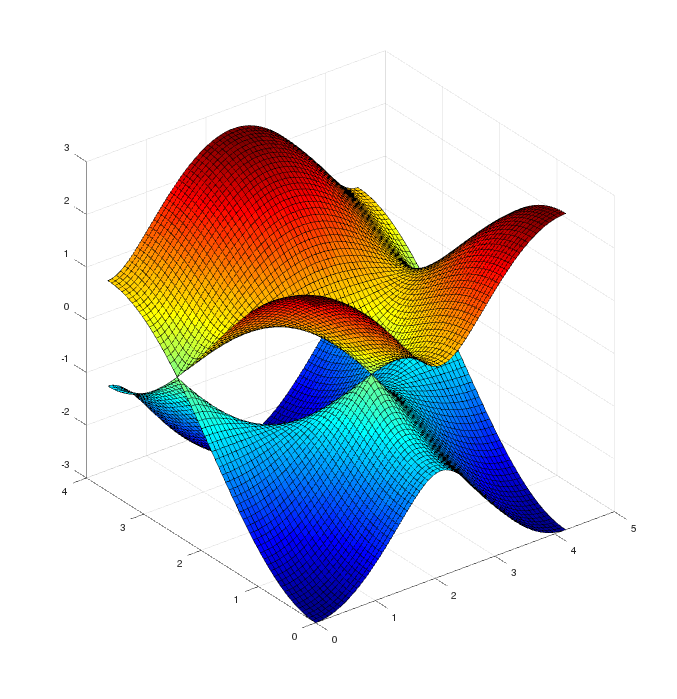
\includegraphics[scale=0.4]{graphics/specgraph.png}
\caption{Spectral bands of $H_{\textrm{km}}$ for $d = 1$ on the fundamental domain $[0,4\pi/3] \times [0,2\pi/\sqrt{3}]$ with $\lambda_{\textrm{nn}} = 1$ and $\lambda_{\textrm{se}} = \lambda_{\textrm{so}} = \lambda_{\textrm{ra}} = 0$}
\label{fig:specgraph}
\end{figure}
\item
   For $\lambda_{\textrm{nn}} \neq 0$, $\lambda_{\textrm{so}} \neq 0$ and $\lambda_{\textrm{ra}} = 0$ we can distinguish two topological phases: the ordinary insulator phase for $\lambda_{\textrm{se}} > 3\sqrt{3}\lambda_{\textrm{so}}$ (see figure \ref{fig:specins}) and the so called \textit{quantum spin hall (QSH)} phase for $\lambda_{\textrm{se}} < 3\sqrt{3}\lambda_{\textrm{so}}$ (see figure \ref{fig:specqsh}). Note that for $\lambda_{\textrm{ra}} = 0$ the third component of the spin is conserved and $H_{\textrm{km}}$ can be written as $H_{\textrm{km}}^{\uparrow} + H_{\textrm{km}}^{\downarrow}$. This means one Hamilton operator for each spin. Associated to each of them is an integer $n^{\uparrow},n^{\downarrow}$ which is the Chern number of $E_{P_{\textrm{km}}^{F}}$ for the according parts of the Hamilton operator as in section \ref{sec:topins}. And though $n^{\uparrow} + n^{\downarrow} = 0$ holds due to time reversal symmetry,
\begin{align*}
  \nu
  &:=
  \frac{n^{\uparrow} - n^{\downarrow}}{2}
  \in
  \mathbb{Z}
\end{align*}
isn't necessarily zero. In fact, according to \cite{f6db8935} we get
\begin{align*}
  I_{\textrm{km}}
  &=
  \nu
  \mod
  2
\end{align*}
In this case a conductance can occur. Namely if $n^{\uparrow} \neq 0$ there is a conductance of spin up electrons and consequently one of spin down electrons since the sum must be zero. This spin conductance is quantized. So one can speak of a \textit{quantized spin Hall\footnote{please note that the physical origin of this phenomenom is the magnetic field due to the spin-orbit coupling} conductance} for $\nu$.
\begin{figure}[H]
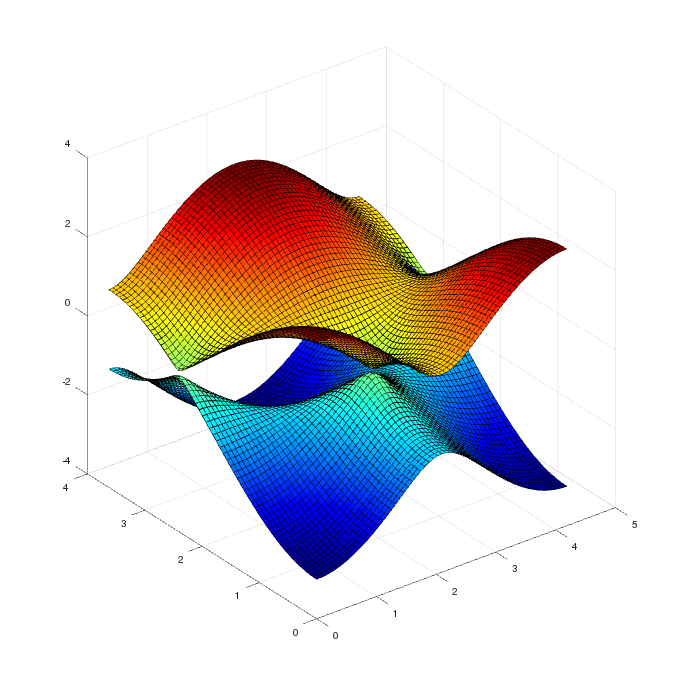
\includegraphics[scale=0.4]{graphics/specins.png}
\caption{Spectral bands of $H_{\textrm{km}}$ for $d = 1$ on the fundamental domain $[0,4\pi/3] \times [0,2\pi/\sqrt{3}]$ with $\lambda_{\textrm{nn}} = 1$, $\lambda_{\textrm{se}} = 0.1$, $\lambda_{\textrm{so}} = 0.006$ and $\lambda_{\textrm{ra}} = 0$}
\label{fig:specins}
\end{figure}
\begin{figure}[H]
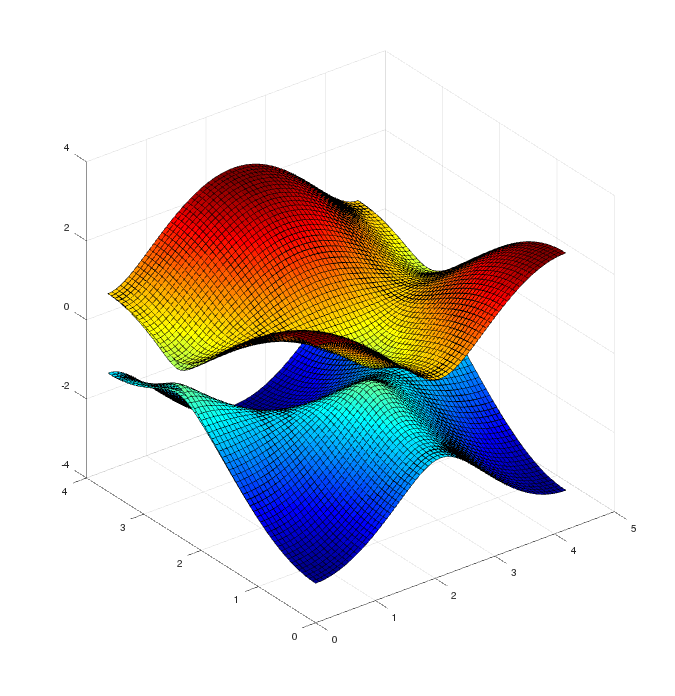
\includegraphics[scale=0.4]{graphics/specqsh.png}
\caption{Spectral bands of $H_{\textrm{km}}$ for $d = 1$ on the fundamental domain $[0,4\pi/3] \times [0,2\pi/\sqrt{3}]$ with $\lambda_{\textrm{nn}} = 1$, $\lambda_{\textrm{se}} = 0.1$, $\lambda_{\textrm{so}} = 0.06$ and $\lambda_{\textrm{ra}} = 0$}
\label{fig:specqsh}
\end{figure}
\item
  In the previous cases we assumed $\lambda_{\textrm{ra}} = 0$. But this is unrealistic and the unavoidably emerging rashba term kills the spin conservation. This makes $\nu$ meaningless. Nevertheless $I_{\textrm{km}}$ stays valid. There exists $x$ satisfying $x < 2\sqrt{3}\lambda_{\textrm{so}}$ such that QSH phase is retained for $0 \leq \lambda_{\textrm{ra}} \leq x$ if it was present for $\lambda_{\textrm{ra}} = 0$ (see figure \ref{fig:specrash}). If $x > 0$ there is still a spin conductance. However, it is not necessarily quantized anymore.
\begin{figure}[H]
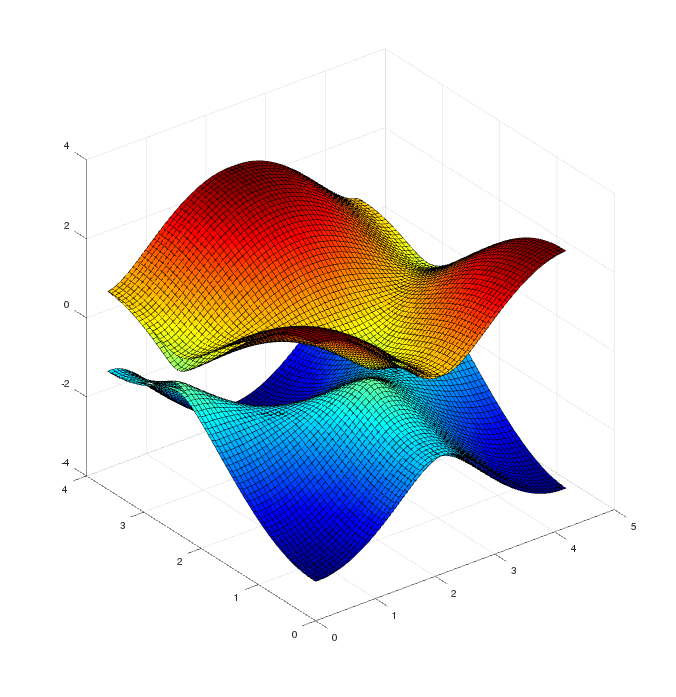
\includegraphics[scale=0.4]{graphics/specrash.png}
\caption{Spectral bands of $H_{\textrm{km}}$ for $d = 1$ on the fundamental domain $[0,4\pi/3] \times [0,2\pi/\sqrt{3}]$ with $\lambda_{\textrm{nn}} = 1$, $\lambda_{\textrm{se}} = 0.1$, $\lambda_{\textrm{so}} = 0.06$, $\lambda_{\textrm{ra}} = 0.05$}
\label{fig:specrash}
\end{figure}
\end{enumerate}
The Kane-Mele model is quite explicit. Indeed, it is explicit enough to implement it what we have done in \href{https://github.com/shtsoft/topins/blob/master/code/kmm.m}{https://github.com/shtsoft/topins/blob/master/code/kmm.m} and used in the above visualization of the energy bands. Another advantage of the implementation is to easily find propositions concerning the physiscs of the Kane-Mele model. Let us demonstrate in a concluding example on the thermodynamic pressure of the Kane-Mele model in an external magnetic field.
\\
\begin{exa}
\label{exa:tdpressure}
This example deals with a conjecture regarding a classical approximation of the Kane-Mele model's thermodynamic pressure in an external magnetic field on the basis of a numerical analysis.
\\
First, an external magnetic field in $e_{3}$ direction is described by the magnetic vector potential
\begin{align*}
  A(y_{1},y_{2})
  &:=
  (By_{2},0)
\end{align*}
for $B \in \mathbb{R}$. It can be incorporated into the Kane-Mele model by substituting the translation operators by so called \textit{magnetic translation}, that is, translation operators as above but with a position dependent \textit{phase $\exp(\mathrm{i}\phi_{i}(x))$}. To this end let $(x,0) := ((x_{1},x_{2}),0) \in \mathrm{C}_{\textrm{km}}$. Then $\gamma_{i}^{x}(t) = x +td_{i}$ for $t \in [0,1]$ and $i =1,2,3$ is a path connecting nearest neighbors and $\phi_{i}$ is given by
\begin{align*}
  \phi_{i}(x)
  =
  \int_{\gamma_{i}^{x}}
  (By_{2},0)
  \mathrm{d}y
  &=
  B
  \int_{0}^{1}
  (x_{2}+t(d_{i} \vert e_{2}),0)
  d_{i}
  \mathrm{d}t
  \\
  &=
  B
  (d_{i} \vert e_{1})
  \int_{0}^{1}
  (x_{2}+t(d_{i} \vert e_{2}))
  \mathrm{d}t
  =
  B
  (d_{i} \vert e_{1})
  x_{2}
  +
  \frac{1}{2}
  B
  (d_{i} \vert e_{1})
  (d_{i} \vert e_{2})
\end{align*}
So substituting the explicit values for $d_{i}$ yields
\begin{align*}
  \phi_{1}(x)
  =
  \frac{dB}{2}
  x_{2}
  -
  \frac{\sqrt{3}d^{2}B}{8}
  &&
  \phi_{2}(x)
  =
  \frac{dB}{2}
  x_{2}
  +
  \frac{\sqrt{3}d^{2}B}{8}
  &&
  \phi_{3}(x)
  =
  -
  dBx_{2}
\end{align*}
and the magnetic translations $T_{d_{i}}^{B}$ are defined by
\begin{align*}
  T_{d_{i}}^{B}(\psi)(x)
  &:=
  \exp(\mathrm{i}\phi_{i}(x))
  T_{d_{i}}(\psi)(x)
\end{align*}
The numerics in \href{https://github.com/shtsoft/topins/blob/master/code/kmm.m}{https://github.com/shtsoft/topins/blob/master/code/kmm.m} suggest
\\
\begin{con}
\label{con:pressofkmm}
Let $B = B_{0} + \varepsilon b$ with $B_{0} \cdot \mathrm{vol}_{2}(\mathbb{R}^{2}/L_{\textrm{km}}) \in 2\pi\mathbb{Z}$, $b \in \mathbb{R}$ and $\varepsilon > 0$. Let further $\beta \in (0,\infty)$, $\mu = 0$ and $(\chi_{m})_{m\in\mathbb{N}^{\times}}$ such that $\chi_{m} \in \mathcal{S}(\mathbb{R}^{2},\mathbb{R})$ has support in $\Lambda_{m} \supset \mathrm{supp}(\chi_{m})$ with $\chi_{m} \vert \Lambda_{m-1} = 1$ if $\Lambda_{m} := [-m,m] \times [-m,m]$. Then the limit
\begin{align*}
  \lim_{\beta \to \infty}
  \beta^{-1}
  \lim_{m\to\infty}
  \frac{\varepsilon^{2}}{\Vert \chi_{m} \Vert_{L_{1}}}
  \mathrm{tr}_{\ell^{2}(\mathrm{C}_{\textrm{km}} \times \mathbb{C}^{2})}
  \left(
    \chi_{m}(\varepsilon x)
    \cdot
    \ln
    \left(
      1
      +
      \exp
      \left(
        -
        \beta
        \left(
          H_{\textrm{km}}^{B}
          -
          \mu
        \right)
      \right)
    \right)
  \right)
\end{align*}
exists and is approximated by
\begin{align*}
  \lim_{\beta \to \infty}
  \frac{1}{4 \cdot \mathrm{vol}_{2}(\mathbb{R}^{2}/L_{\textrm{km}}^{\prime})}
  \sum_{i=0}^{3}
  \int_{\mathbb{R}^{2}/L_{\textrm{km}}^{\prime}}
  \left(
    1
    +
    \varepsilon
    b
    \Omega_{(i)}
  \right)
  \ln
  \left(
    1
    +
    \exp
    \left(
      -
      \beta
      \left(
        h_{(i)}
        -
        \mu
      \right)
    \right)
  \right)
  \mathrm{d}k
  +
  \mathcal{O}(\varepsilon^{2})
\end{align*}
for $\varepsilon$ small enough where
\begin{align*}
  \Omega_{(i)}(k)
  &:=
  -
  \mathrm{i}
  \cdot
  \mathrm{tr}_{\mathbb{C}^{4}}
  \left(
    \tilde{P}_{\textrm{km}}^{\lbrace i \rbrace}(k)
    \left[
      \partial_{1}
      \tilde{P}_{\textrm{km}}^{\lbrace i \rbrace}(k),
      \partial_{2}
      \tilde{P}_{\textrm{km}}^{\lbrace i \rbrace}(k)
    \right]
  \right)
  \\
  h_{(i)}(k)
  &:=
  E_{i}(k)
  +
  \varepsilon
  b
  \cdot
  \mathrm{Im}
  \left(
    \mathrm{tr}_{\mathbb{C}^{4}}
    \left(
      \tilde{P}_{\textrm{km}}^{\lbrace i \rbrace}(k)
      \partial_{1}
      \tilde{P}_{\textrm{km}}^{\lbrace i \rbrace}(k)
      \left(
        \tilde{H}_{\textrm{km}}(k)
        -
        E_{i}(k)
        \cdot
        1_{\mathbb{C}^{4 \times 4}}
      \right)
      \partial_{2}
      \tilde{P}_{\textrm{km}}^{\lbrace i \rbrace}(k)
    \right)
  \right)
\end{align*}
\phantom{proven}
\hfill
$\square$
\end{con}
\phantom{proven}
\hfill
$\square$
\end{exa}



\nocite{wiki-pedia0en}

\bibliographystyle{alpha}
\bibliography{bib}

\end{document}
